\chapter{Background and Literature Review}

\epigraph{\itshape People generally see what they look for, and hear what they listen for.}{---Harper Lee}

The below section lays out the theoretical background on \acrfull{uatr} and conducts a broad survey of the most influential literature in the field. It also presents a detailed summary of the current publicly available datasets for use in \acrshort{uatr} research.

\section{Foundational principles of sonar systems}

The aim of this section is to provide the unfamiliar reader with a foundational understanding of underwater acoustics and sonar, essential for comprehending the primary content of this thesis. First, we contextualise our work by giving a brief overview of the historical development of acoustics and sonar technologies. Then, since sonar systems are fundamentally based on the principles of underwater signal propagation, we introduce key concepts and challenges encountered when working with underwater signals such as signal attenuation, multipath propagation, and ambient noise. Following this, we cover both active and passive sonar systems, outlining their mechanisms and the sonar equations that define their operation. Finally, we introduce a few applications of sonar systems including an introduction to the primary topic of this thesis, underwater acoustic target recognition.

\subsection{Historical development of underwater acoustics and sonar}\label{sec:uw-history}

In 1490, polymath Leonardo da Vinci conducted an early experiment with the propagation of sound waves underwater and noted the following observation:
\begin{quote}
    If you cause your ship to stop and place the head of a long tube in the water and place the outer extremity to your ear, you will hear ships at a great distance from you. \cite{urick_principles_1975}
\end{quote}
One could call this the birth of the study of underwater acoustics, as da Vinci's observation over 500 years ago is the same basic principle used in underwater sonar systems today.

Over the next four centuries, it would take the combined effort of many great minds to lay the foundations of acoustic theory. Marin Mersenne (of Mersenne primes fame) formalised the theory of vibrating strings and harmonics in 1636 \cite{mersenne_harmonie_1957}. Isaac Newton then presented the first mathematical theory of sound propagation in air in his 1687 work \textit{Principia} \cite{newton_principia_2013}. In the early 18th century, Brook Taylor, along with Leonhard Euler, Jean d'Alembert, and Daniel Bernoulli, sought to demonstrate that any acoustic vibration could be expressed as a superposition of sinusoidal vibrations, a problem fully solved by J.L. Lagrange in 1759 \cite{darrigol_acoustic_2007}. Georg Ohm further contributed with his law of hearing in 1843 \cite{dixon_ward_musical_1970}, inspiring Hermann von Helmholtz's cornerstone 1863 work \textit{On the Sensations of Tone} \cite{helmholtz_sensations_1954} which focused on the perception of sound. Finally, Nobel laureate Lord Rayleigh formalised the wave equation in his seminal 1877 text, \textit{The Theory of Sound} \cite{rayleigh_theory_2011}, cementing the theoretical framework for modern acoustics \cite{vaccaro_past_1998}.

Ultimately, however, it was the sinking of the Titanic in 1912 that provided the financial and industrial incentives for the development of new naval navigation technologies. Canadian engineer Reginald Fessenden responded by creating the first primitive sonar system in 1914. He developed an early kind of transducer (a device capable of both sending and receiving sound) which he called the \textit{Fessenden Oscillator}. Resembling a large loudspeaker, the device used a vibrating copper tube and steel diaphragm to produce a focused sound wave. During a test in icy waters, Fessenden lowered the oscillator into the ocean and sent out a signal. The sound waves struck an iceberg and returned as an echo just over a second later. This marked the beginnings of  what we now know as \textit{active sonar}, the underwater equivalent of radar \cite{dinneen_reginald_2020, vaccaro_past_1998}.

World War I further catalysed the rapid advancement of sonar technology. Extending Fessenden's work, French physicist Paul Langevin developed the first sonar system to use a crystal transducer, which sent and received sound waves using the piezoelectric effect in contrast to Fessenden's mechanical implementation. This innovation, driven by the need to detect German U-boats, represented a significant leap forward from Fessenden's earlier work \cite{rodriguez_fundamentals_2023}. 

World War II and the Cold War continued to propel sonar development. One of the key focuses was the development of sonar systems capable of detecting enemy submarines from long distances, even in complex and noisy underwater environments. Early on, anti-submarine warfare was dominated by the use of activate sonar systems such as ASDIC (derived from Anti-Submarine Detection Investigation Committee), which worked in a similar fashion to Fessenden and Langevin's work \cite{helgason_asdic_2011}. However, the advent of \textit{passive} sonar, which relied on listening for sounds rather than actively emitting signals, became a major focus later on in this period. Passive sonar allowed submarines and other vessels to detect enemy movements without giving away their own location, making it a vital tool in the Cold War's ``silent'' naval battles. 

One of the key discoveries which allowed passive sonar to work so well in performing passive sonar surveillance was the \acrfull{sofar} channel, discovered in 1944 by ocean scientists Ewing and Worzel. \acrshort{sofar} works by taking advantage of the ocean’s layered structure, where sound waves emitted at a certain depth bounce between layers of water with different temperatures and salinity. This up-and-down bending of low-frequency soundwaves allows them to travel vast distances with minimal energy loss \cite{national_oceanic_and_atmospheric_association_what_2024}. Building on this discovery, the U.S. Navy developed the \acrfull{sosus} in the 1950s, which deployed arrays of hydrophones in the \acrshort{sofar} sound channel to track Soviet submarines. The system was highly effective, enabling long-range detection in noisy environments and playing a pivotal role in Cold War anti-submarine warfare. Additionally, \acrshort{sosus} arrays helped scientists study oceanic phenomena like whale calls and deep-sea currents \cite{morin_history_nodate}.

Other technological improvements in the early stages of the Cold War included advances in array processing, where multiple sensors were used to improve signal detection, enhancing the range and accuracy of sonar systems. Additionally, algorithms were developed to filter useful sonar signals from background noise, employing methods like adaptive beamforming to focus on specific directions and improve the signal-to-noise ratio. The rise of scientific computing and the transition to digital signal processing further revolutionised the field, enabling more advanced techniques such as time-delay estimation and spectral analysis.

Progress in underwater signal processing during the 1970s and early 1980s was closely linked to advancements in general signal processing techniques. Researchers in underwater acoustics focused on improving high-resolution signal processing -- that is, the ability to separate signals from sources with nearly identical frequencies or positions, such as two nearby ships or objects \cite{vaccaro_past_1998}. These efforts greatly enhanced the precision of sonar systems, enabling them to detect underwater objects more effectively, even in noisy or interference-heavy environments.

It was during the 1980s and 1990s that the field of \textit{automatic} underwater acoustic classification, which this thesis is rooted in, truly came into its own. This shift was largely driven by the Cold War, when sonar engineers and submarine builders became acutely aware of the need to make ships ``quieter.'' As a result, vessel-radiated noise was reduced, making it harder for sonar operators to detect man-made targets. According to Vaccaro et al. in their 1998 review of the field:

\begin{quote}
    ...the quieting of targets requires raising the threshold of detectability, which in turn increases the rate of false alarms and thus overwhelms the human operator. Automating these tasks by extracting classification features that cue the operator to relevant targets is important. \cite[46]{vaccaro_past_1998}
\end{quote}

Finally, the 2000s saw significant advances in environmental applications of underwater acoustics. Many studies during this period greatly focused on the growing concerns over anthropogenic underwater noise from shipping, military sonar, and industrial activities, which pose threats to marine ecosystems by interfering with the communication and behaviour of aquatic life \cite{erbe_underwater_2002, slabbekoorn_noisy_2010, wysocki_diversity_2007}.

Now that the field of underwater acoustics has been grounded in history, we shall continue by presenting a brief summary of the relevant theoretical concepts in the field.


\subsection{Signal propagation in the underwater environment}\label{subsec:sig-prop-uw-env}

Let us begin with the most fundamental concept in underwater acoustics -- sound. Being a mechanical wave, the propagation of sound relies on the density and elasticity of the medium it travels through. In turn, the density and elasticity of water is influenced by factors such as temperature, salinity, and pressure \cite{sinay_diving_2024}. Hence, the speed of sound in water has many complex formulations \cite{leroy_new_2008}. A simplified, empirical formula for calculating the speed of sound, $c$, in the ocean based on temperature $T$ (in degrees Celsius), depth $z$ (in meters), and salinity $S$ (in parts per thousand) is given by \cite{abraham_underwater_2019}: 
\begin{equation}
c = 1449.2 + 4.6T + 0.055T^2 + 1.39(S - 35) + 0.016z \label{eq:speed-of-sound-in-water}
\end{equation}

The speed of sound in water plays a crucial role in various underwater acoustic phenomena. One of the most significant of these is refraction, which occurs when sound waves pass through layers of water with different sound speeds \cite{urick_principles_1975}. Refraction causes sound waves to bend as they travel through these layers, following Snell's law:
\begin{equation}
    \frac{\cos \theta_1}{c_1} = \frac{\cos \theta_2}{c_2}\label{eq:snells}
\end{equation}
where $\theta_1$ and $\theta_2$ are the angles of incidence and refraction, and $c_1$ and $c_2$ are the sound speeds in the two layers, respectively \cite{domingos_survey_2022}.  The combination of Equations \ref{eq:speed-of-sound-in-water} and \ref{eq:snells} reveals a crucial phenomenon in underwater acoustics: sound waves bend towards cooler regions of water. This refraction effect requires adapting sound profiles based on temperature variations, such as between geographic regions or different times of the year \cite[3]{domingos_survey_2022}. Moreover, under certain conditions, acoustic refraction can create \textit{shadow zones} -- areas where sound waves cannot penetrate, resulting in signal loss \cite{vaccaro_past_1998}.

Related to refraction is the concept of reflection. When sound waves encounter boundaries such as the sea surface or seafloor, part of the acoustic energy is reflected. The amount of reflection depends on the difference between the speed of sound in water and the boundary material, a value called the \textit{acoustic impedence mismatch} \cite{jackson_high-frequency_2007}. Reflection is a key concept in several applications of underwater acoustics, particularly in the field of sonar imaging. 

There are several other factors besides acoustic refraction which can cause signal attenuation in the underwater environment, including absorption, scattering, and geometrical spreading losses. Absorption loss occurs when acoustic energy is converted into thermal energy as it travels through seawater, with its extent depending on variables such as salinity, temperature, pH, pressure, and signal frequency. This absorption can range from around 0.07 dB/km at 1 kHz to 9.0 dB/km at 40 kHz, making high-frequency signals particularly susceptible to loss \cite{bjorno_applied_2017, vaccaro_past_1998}. Scattering is another significant source of attenuation as objects like fish, bubbles, rocks, and surface waves disperse sound energy in all directions, effectively masking the signal and complicating detection \cite{bjorno_applied_2017}. Additionally, frequency-independent spreading losses arise from geometrical spreading, where signal energy decays with distance. In shorter ranges, spherical spreading results in a decay rate proportional to $1/R^2$, while at longer ranges, cylindrical spreading causes a $1/R$ decay, where $R$ is the distance from the source \cite{vaccaro_past_1998}.

In addition to these sources of signal loss, underwater signal propagation is further complicated by \textit{multipath propagation}. This phenomenon arises when sound waves reflect off the sea surface or seabed and refract through different layers of water, each with varying sound speeds. These interactions cause the signal to split and travel along multiple paths from the source to the receiver (Figure \ref{fig:multipath}). As a result, several versions of the same signal arrive at the receiver at different times, causing delay spreads and signal distortion. The extent of these delays varies depending on the environment. For example, in shallow waters (less than 10 meters deep), delay spreads can reach up to 10 milliseconds, while in deeper waters, these delays may extend beyond 300 milliseconds \cite{vaccaro_past_1998}. This variation in arrival times can complicate the detection and identification of underwater objects.

\begin{figure}[htbp]
    \centering
    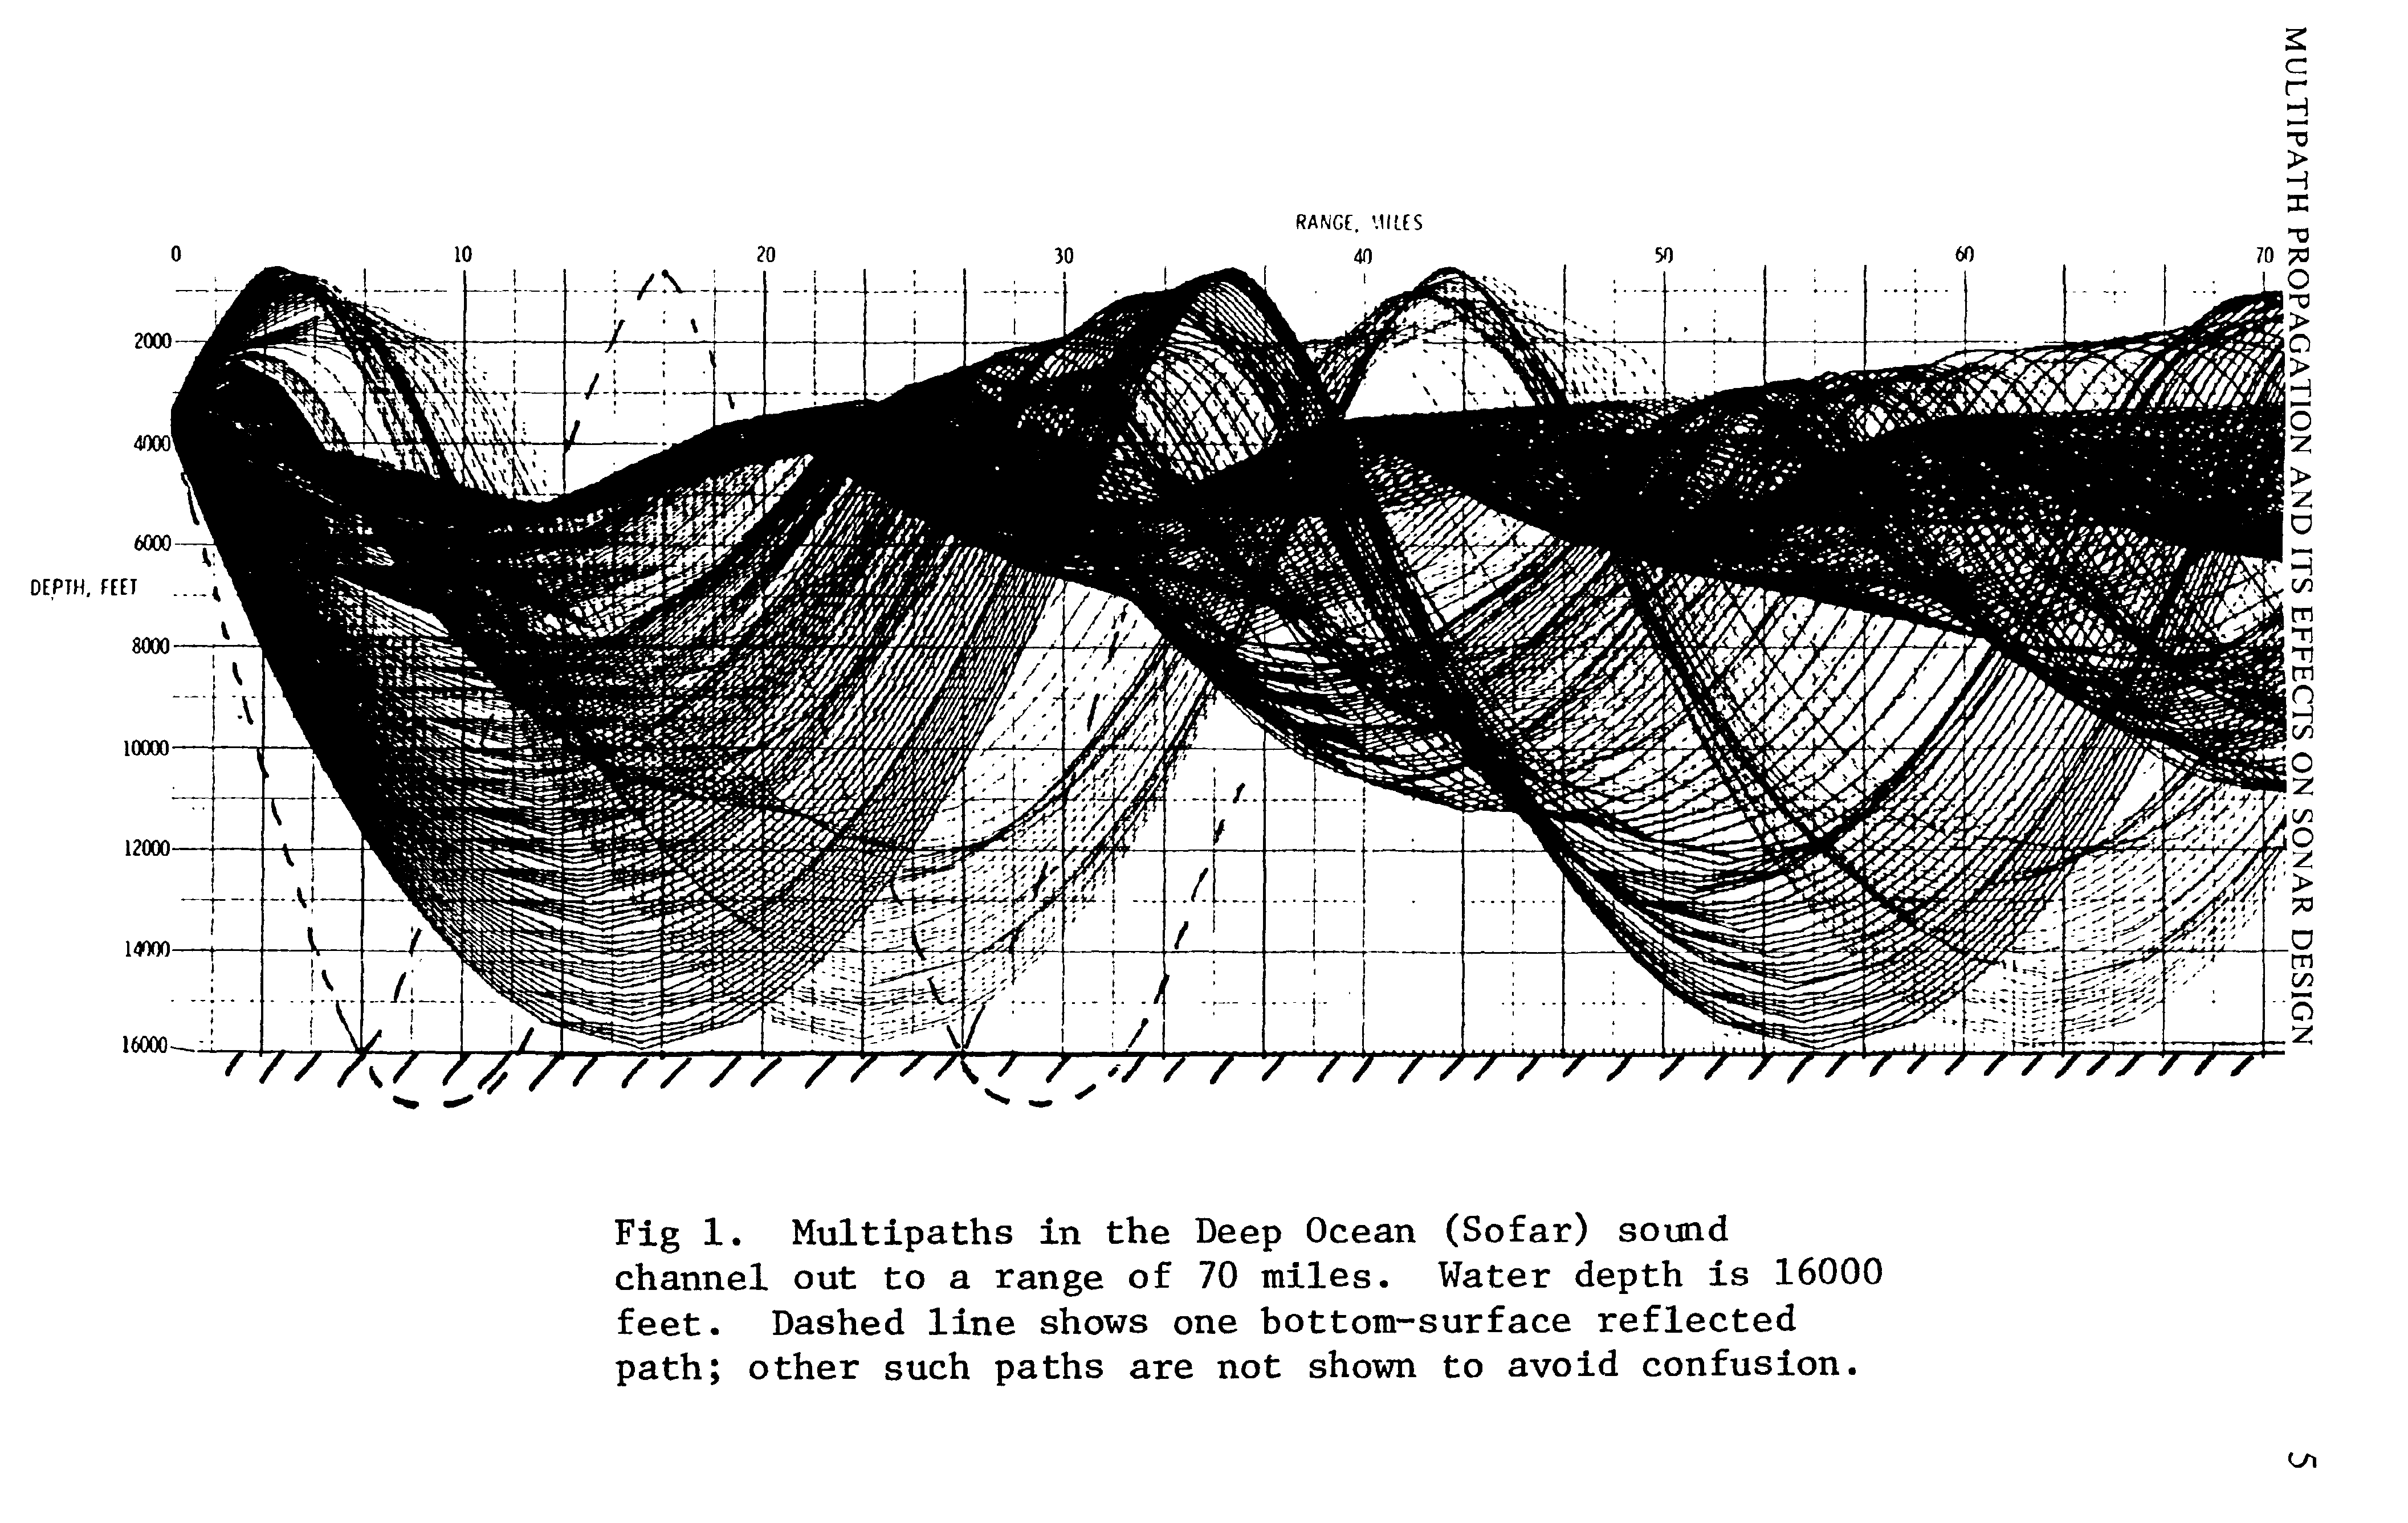
\includegraphics[trim={0 20cm 3cm 0},clip,width=\textwidth]{img/ch2/multipath.png}
    \caption{Figure depicting the multipaths in the SOFAR band, obtained from \cite[Fig. 1]{tacconi_multipath_1977}}
    \label{fig:multipath}
\end{figure}

In summary, the underwater environment poses significant challenges for acoustic signal propagation due to a broad range of factors. Changes in temperature, salinity, and pressure affect the speed of sound, leading to phenomena such as refraction and shadow zones. Absorption and scattering of sound by marine life and other underwater phenomena contribute to signal attenuation, especially at higher frequencies. Multipath propagation results in delays and signal distortion, making the detection and classification of underwater objects particularly challenging. Collectively, these factors create a highly complex underwater acoustic landscape.

\subsection{Sources of noise in underwater acoustics}\label{subsec:noise}

One of the key challenges in underwater signal processing is noise, as it can obscure the original data and complicate accurate interpretation. In fact, due to the extreme complexities of the underwater environment (as described in the previous section), noise is generally a greater problem for signals underwater as compared to in-air signals. There are three main sources of underwater noise: vessel noise, ambient noise, and thermal noise \cite{waite_sonar_2002}. Each source introduces distinct challenges for acoustic signal detection and analysis. This section aims to provide a comprehensive summary of these sources.

\subsubsection{Vessel noise}

There are three main sources of noise from a vessel, which, when summed, form the `self-noise' of a sonar system \cite{ross_mechanics_1976}. Each of these have fairly characteristic frequency bands and are heavily dependent on the vessel speed \cite{zak_ships_2008}. 

Machinery noise originates from various mechanical systems on a vessel, including engines, pumps, and rotating equipment. These mechanical systems create vibrations that are transmitted to the ship’s hull, which then acts as a medium for noise radiation. Machinery noise can be divided into discrete and continuous categories. Discrete noise is typically produced by components such as shafts, motor armatures, and turbine blades, resulting in a tonal spectrum dominated by fundamental frequencies and their harmonics, generated by the vibrating machinery. On the other hand, continuous noise is associated with repetitive impacts, such as explosions in engine cylinders, and the friction and turbulence occurring in pumps, pipes, and bearings. These processes create persistent noise that adds to the underwater soundscape \cite{zak_ships_2008, chin-hsing_classification_1998}.

Hydrodynamic noise results from the ship's movement through water. As the ship moves, the water flow around the hull generates pressure variations, typically manifests as low-frequency, broadband noise, encompassing a wide range of frequencies. This noise becomes more pronounced at higher vessel speeds or in rougher sea conditions, as the level of turbulence increases with both speed and environmental factors \cite{bjorno_applied_2017}.

Propeller noise is another significant source of underwater noise, arising from the interaction between the propellers and the surrounding water. This noise is primarily categorised into cavitation noise and blade noise. Cavitation occurs when low-pressure areas around the edges of the propeller blades cause bubbles to form. These bubbles then collapse, producing high-frequency, broadband noise. In contrast, blade noise is produced by the rotation of the propeller blades, where factors such as the blade’s thickness and the loading exerted on it generate narrow-band, low-frequency sounds. Propeller noise, particularly cavitation, is often a dominant contributor to underwater vessel noise, especially at higher speeds or under heavy loads \cite{malinowski_underwater_2001}.

Generally speaking, machinery noise is dominant at slow speeds (up to 10 knots), hydrodynamic noise is dominant at medium speeds (10 to 20 knots), and propeller noise begins to dominate above this \cite{waite_sonar_2002}. 

\subsubsection{Ambient noise}

\begin{figure}[p]
    \centering
    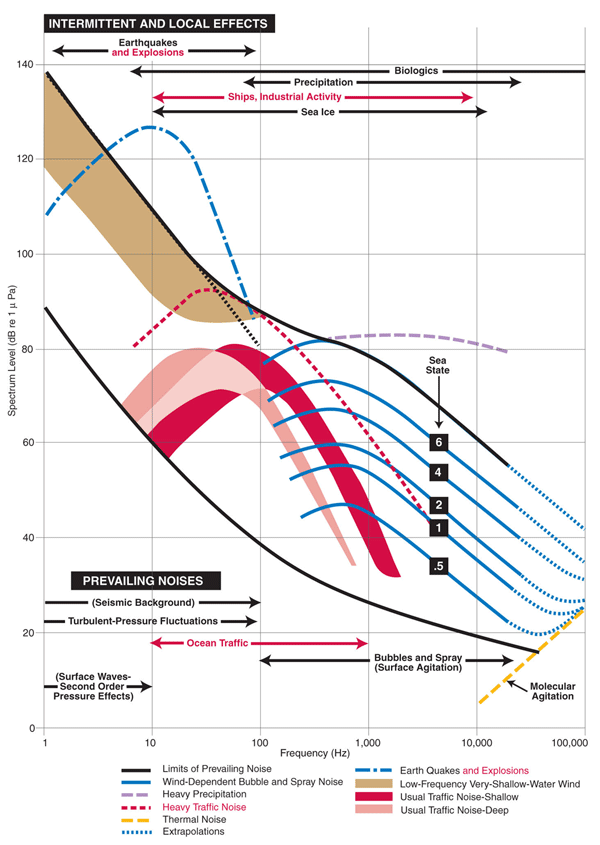
\includegraphics[width=0.9\textwidth]{img/ch1/uw_noise.png}
    \caption{Sources of underwater noise and their approximate frequency ranges, obtained from \cite{knowlton_what_nodate}, data originally from \cite{wenz_review_1972}.}
    \label{fig:uw-noise}
\end{figure}

Ambient noise in underwater environments is generated from a range of natural and anthropogenic (human-induced) sources, creating a complex acoustic landscape. Below is a brief summary of some of the major sources of such noise; see Figure \ref{fig:uw-noise} for a more comprehensive overview of the frequency ranges of each source.

Seismic activity, such as underwater earthquakes (seaquakes) and volcanic eruptions, contributes significantly to low-frequency noise, especially below 20 Hz. These geophysical events introduce deep, powerful sounds into the ocean, which can travel long distances and influence ambient noise levels in various marine regions \cite{knowlton_what_nodate}.

Shipping vessels are another major source of ambient noise, particularly within the 20-500 Hz range. As global shipping traffic has increased \cite{andrew_ocean_2002}, the noise generated by distant cargo ships, primarily through propeller cavitation, has become a dominant contributor to ambient noise in this frequency range. The cumulative effect of numerous ships radiating sound into the ocean is substantial, raising the baseline level of ocean noise \cite{ross_mechanics_1976}.

Hydrostatic effects, such as tidal movements, along with weather-related phenomena like precipitation, contribute to higher frequency noise, ranging from 500 Hz to 100,000 Hz. Wind, rain, hail, and the formation of bubbles from breaking waves all play roles in generating noise at these higher frequencies. Various factors, such as droplet size and shape, affect the acoustic characteristics of this type of noise, making it highly variable and dependent on environmental conditions \cite{medwin_bubble_1989, franz_splashes_1959, dahl_underwater_2007}.

Biological activity is a major contributor to ambient underwater noise levels. Sounds produced by marine life cover a wide frequency range \cite{bjorno_applied_2017}. In subtropical shallow waters worldwide, the dominant source of ambient noise often comes from the biological sounds of fish, dolphins, whales, and snapping shrimp \cite{cato_ultrasonic_1992}. The study of these sounds, known as bioacoustics, has provided valuable insights into animal behavior. For instance, it has allowed us to characterise the different sounds whales use for communication, predator-prey interactions, and social bonding, such as their ``whistles,'' ``clicks,'' and ``pulsed calls'' \cite{richardson_marine_1995}. Bioacoustics has also shed light on the mechanism behind the noise produced by snapping shrimp, with studies exploring the evolutionary and physical factors that contribute to their distinctive sound \cite{patek_evolutionary_2018, lohse_snapping_2001, ritzmann_snapping_1973}.

Finally, other anthropogenic activities, such as construction, offshore drilling, and underwater mining, also contribute to ambient noise. These activities can introduce a broad range of noise frequencies and intensities, exacerbating the overall noise pollution in marine environments. 

\subsubsection{Thermal noise}
    In the absence of ambient and vessel noise, the underlying noise level is determined by thermal noise. Thermal noise is inherent in any electrical receiving system, including sonar receivers. This noise is generated by the agitation of electrons in the electrical components, which translates to pressure fluctuations at the face of the hydrophone \cite{waite_sonar_2002}. Mellen's expression for thermal noise is: $N_\text{thermal} = -15 + 20 \log f$, where $f$ is the frequency in kilohertz. Mellen's expression highlights that thermal noise increases with frequency, impacting the sensitivity and performance of sonar systems at different operational frequencies \cite{bjorno_applied_2017}. Thermal noise dominates at frequencies around 100,000 Hz \cite{dahl_underwater_2007}.

\subsection{How does sonar work?}\label{subsec:sonar-working}

Now that the fundamental principles of underwater sound propagation have been laid, it is time to briefly cover the operation of sonar systems.

Sonar operates by converting acoustic energy into electrical signals, and vice versa, through specialised underwater transducers known as hydrophones \cite{waite_sonar_2002, rodriguez_fundamentals_2023, abraham_underwater_2019}. In active sonar, the system first converts an electrical signal into an acoustic pulse using a transducer. The pulse travels through the water until it reflects off an object or the seafloor. The returning reflected sound wave, or echo, is captured by the hydrophones, which transform the acoustic energy back into electrical signals for analysis. This allows active sonar systems to determine both the range and orientation of underwater objects. Active sonar is commonly used in applications requiring high-resolution imaging, such as mapping the seafloor and identifying shipwrecks.

In contrast, passive sonar operates by listening for sounds naturally produced in the underwater environment, such as those from ship engines, propellers, biological sources, or geological activity. Passive sonar systems do not emit sound waves themselves, making them highly advantageous in military operations for stealth purposes, as they cannot be detected. However, unlike active sonar, passive systems cannot directly measure the range of an object unless multiple sensors are used to triangulate the sound source.

The performance of sonar systems, particularly in terms of detection, is typically quantified using the \textit{sonar equations} \cite{abraham_underwater_2019, waite_sonar_2002}. These equations estimate the \acrfull{snr} for both passive and active sonar systems by accounting for various factors such as source level (SL), propagation loss (PL), noise level (NL), and array gain (AG), all of which are expressed in decibels. For passive sonar systems, the SNR is calculated using the equation:
\begin{equation}
    SNR_\text{passive} = SL - PL - NL + AG
\end{equation}
In active sonar systems, additional variables such as target strength (TS) and further transmission losses (TL) are considered:
\begin{equation}
    SNR_\text{active} = SL - 2TL + TS - NL + AG
\end{equation}

\subsection{Applications of sonar systems}
Sonar technology has a wide range of applications, many of which have seen significant advancements through the incorporation of \acrlong{ml} techniques \cite{bianco_machine_2019}. One significant application is underwater source localisation, where sonar systems detect and triangulate the position of sound sources such as submarines or marine animals using arrays of hydrophones \cite{su_review_2020, wang_underwater_2018, zhang_underwater_2018}. By analysing the time difference of arrival of sound waves at different hydrophones, these systems can pinpoint a target's location, making it incredibly useful for military operations and marine biology studies. Another related application is the estimation of the direction of arrival of sound waves, which helps determine the angle from which the sound is coming \cite{ozanich_feedforward_2020, liu_doa_2021, li_deep_2022, cao_deep_2016}. Using advanced beamforming techniques in conjunction with \acrlong{ml}, sonar systems can isolate specific sounds from background noise, providing crucial information in defence and navigation scenarios. 

Beyond localisation and direction estimation, sonar also has more specialised applications. For instance, by analysing the sound generated by wind-driven processes such as breaking waves, it is possible to estimate wind speed over the ocean \cite{cauchy_wind_2018}. This is especially useful for remote areas where traditional meteorological instruments cannot be deployed. In bioacoustics, sonar is employed to monitor the behavior and movement of marine species, offering a non-invasive way to study endangered populations \cite{cato_ultrasonic_1992, richardson_marine_1995, patek_evolutionary_2018, lohse_snapping_2001, ritzmann_snapping_1973}. 

\subsubsection{Underwater acoustic target recognition}\label{subsubsec:uatr-intro}

A major application of sonar systems is \acrfull{uatr}, which forms the central focus of this work. Simply put, \acrshort{uatr} is the analysis of a sonar signal with the aim of determining its source. The sonar signal can either be active or passive, however, as described in Section \ref{sec:uw-history} as well as in \cite{mishachandar_diverse_2021}, most applications nowadays rely on passive sonar in order to limit self-detectability as well as harm to sea life. The techniques used for this analysis can be split into two categories: the conventional approach using classical signal processing tools and the \acrfull{ml} approach.

In conventional underwater acoustic target recognition, human sonar operators are responsible for analysing real-time acoustic data to detect and classify underwater objects. The process begins as described in Section \ref{subsec:sonar-working}, with sonar systems detecting sound waves through arrays of hydrophones and converting the acoustic signals into electrical signals. These electrical signals then find their way onto two main interfaces: the broadband display and the narrowband display.

\begin{figure}[htbp]
    \centering
    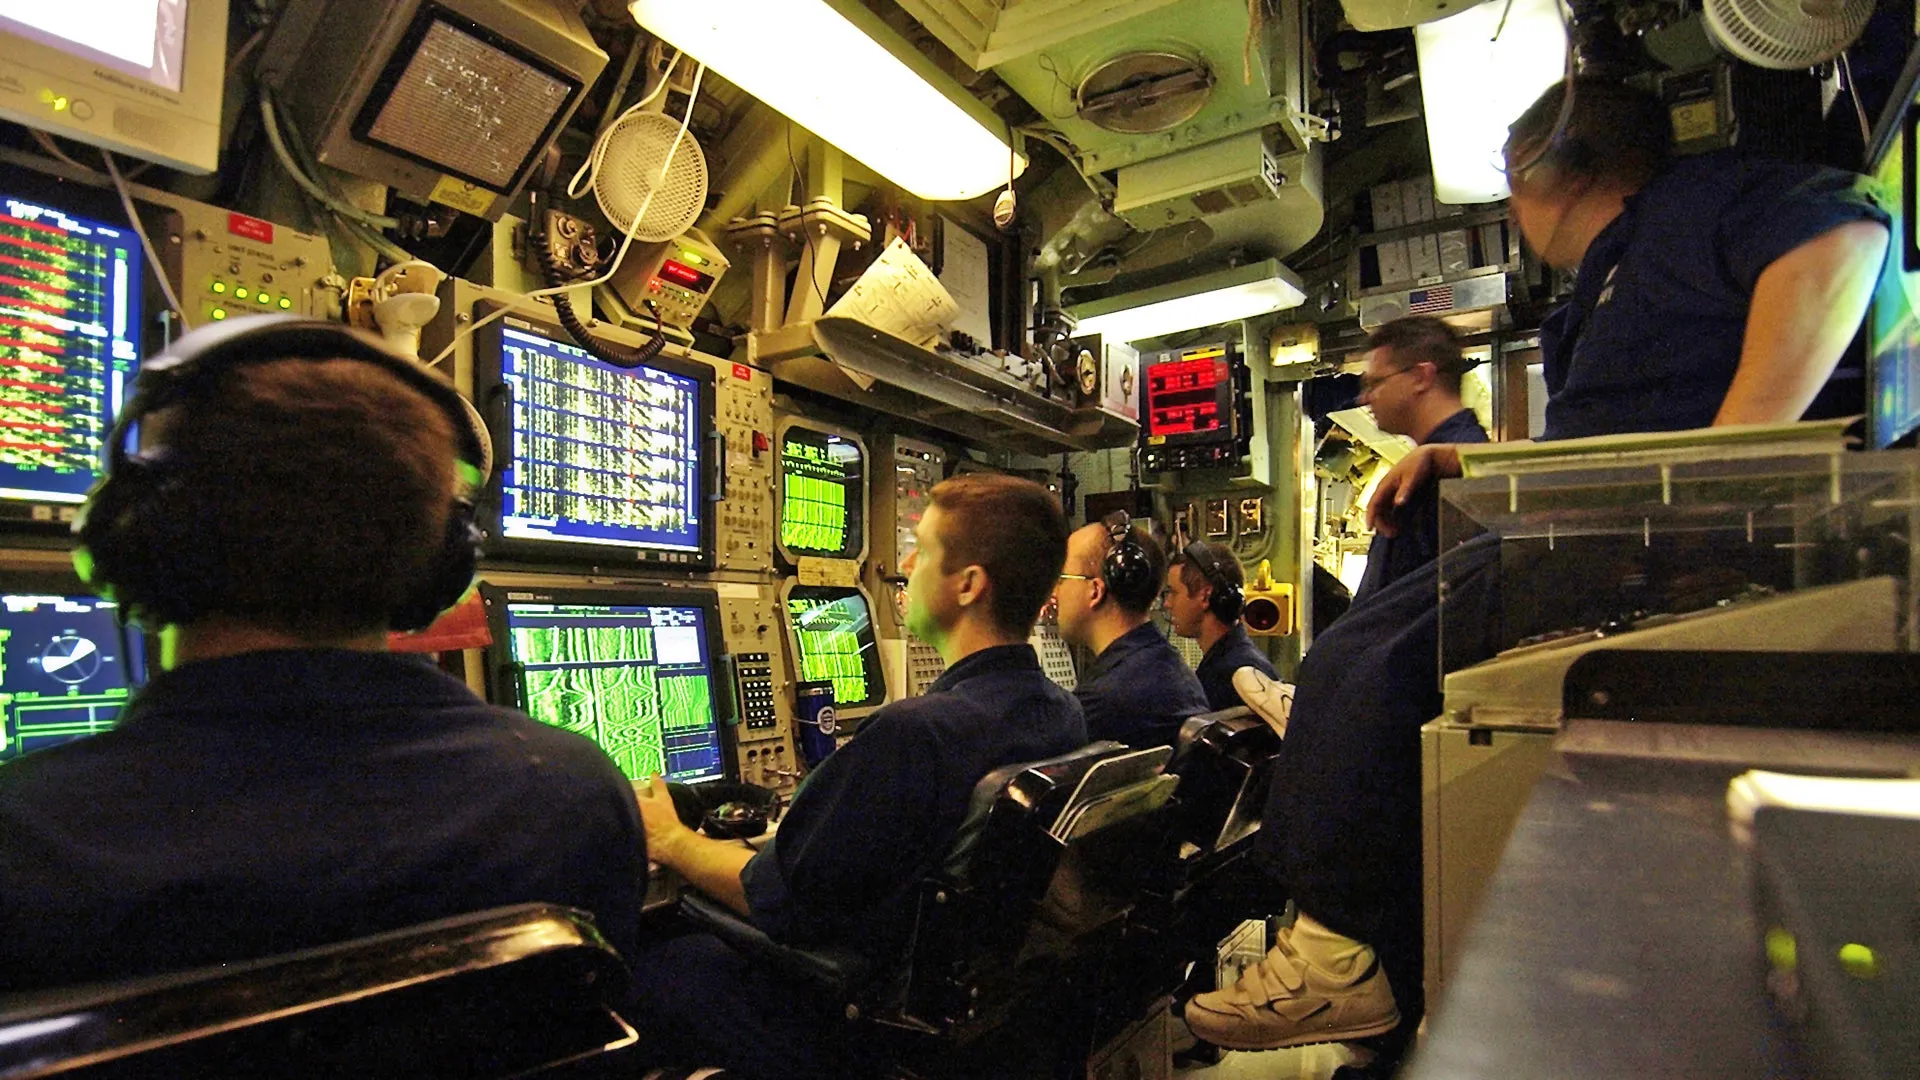
\includegraphics[width=\textwidth]{img/ch2/sonar_operator.png}
    \caption{Sonar operators observing broadband and narrowband displays, obtained from \cite{amick_how_2020}.}
    \label{fig:enter-label}
\end{figure}

The broadband display, often referred to as the ``waterfall display'', displays the total acoustic energy received from the hydrophone array with the latest data ``cascading'' from the top of the screen. This interface allows operators to detect spikes in acoustic energy which could indicate the presence of a target. At this stage, operators observe the different bearings (the direction of the signal relative to the vessel) of the incoming signal and assign it to some broad classification based on their initial impressions, such as biological sound, seismic activity, or vessel noise.

Once a general classification is made, sonar operators transition to the narrowband display, where the broadband signal is divided into its component frequencies through the use of a Fourier transform. Since each object produces distinct spectral characteristics (as discussed in Section \ref{subsec:noise}), operators draw upon various conventional signal processing concepts such as harmonics and modulation patterns to analyse these frequency components in order to classify the incoming signal.

For example, the harmonic structure of mechanical noise generated by a ship's engine or propeller is distinct and recognisable due to its periodic nature, resulting in a clear pattern of fundamental frequencies and their harmonics \cite{chin-hsing_classification_1998}. In contrast, the random noise produced by environmental factors like wind, waves, or marine life is more dispersed across the spectrum, often lacking this periodicity. Operators also look for modulation patterns (changes in amplitude or frequency over time) that may reveal whether the sound is coming from a rotating propeller, hydraulic machinery, or other mechanical components. The operator may also apply band-pass filters to isolate frequencies associated with specific targets, such as the \acrfull{lofar} technique, which focuses on low-frequency sounds characteristic of large vessels. This in-depth spectral analysis typically takes between 30 to 60 seconds, during which operators confirm or revise their initial broad classification \cite{amick_how_2020}.

It is widely accepted that the job of a sonar operator is a challenging task. In high-contact environments, operators face the challenge of managing multiple potential targets simultaneously. They must continuously verify bearings and frequencies, ensuring that the sonar system maintains a reliable track on all contacts. This task is mentally demanding, and sonar watches can last for up to six hours, requiring intense concentration from operators. In addition, due to the inherent setting of the job, sonar operators never truly know that their classification is correct! These are just a few compelling reasons as to why the conventional approach to \acrshort{uatr} continues to dominate in today’s naval operations despite being much more resource-intensive. The expertise, intuition, inferential comprehension, and real-time decision making ability of sonar operators provides a level of accuracy and reliability in vessel classification that no \acrshort{ai} system has fully replaced.

It is important to reflect on this in order to appreciate the inherent limitations of applying \acrshort{ai} techniques like \acrlong{ml} to \acrshort{uatr}. Most modern \acrshort{ai} methods are designed to create \textit{rational agents} -- machines that \textit{act rationally} and ``do the right thing'' by making decisions that maximise some performance metric. For example, \acrlong{ml} models aim to uncover underlying patterns in datasets and optimise their predictions by minimising error through a loss function. This is fundamentally different from the earlier, \textit{human-centred} approaches to \acrshort{ai}, which sought to build systems that could think or act like humans (Table \ref{tab:ai-approaches}) \cite{carnegie_mellon_university_human_2001, russell_artificial_2021}\footnote{See Section \ref{subsec:ai-history} for more on the historical development of \acrshort{ai}.}.

\begin{table}[htbp]
\centering
\begin{tabular}{cc}
\toprule
\textbf{Human-centred approach} & \textbf{Rationality-centred approach} \\ \midrule
Think like humans & Think rationally \\
Act like humans & Act rationally \\ \bottomrule
\end{tabular}
\caption{The four historical perspectives of artificial intelligence proposed by Russell and Norvig \cite{russell_artificial_2021}.}
\label{tab:ai-approaches}
\end{table}

This distinction matters because \acrshort{uatr} is a field that inherently benefits from human abilities such as inference, intuition, context-driven decision-making, and problem-solving. As discussed previously in this section, the underwater acoustic environment is incredibly complex and dynamic. Ambient background noise levels can change drastically within hours, properties such as reflection, refraction, signal attenuation and multipath propagation introduce complexities with signal propagation, and the qualities of sound can differ based on numerous factors such as temperature, salinity and pressure. In such a challenging environment, thinking like a human by synthesising diverse streams of information, including past experience, environmental context, and indirect clues, to form a probable classification for an incoming signal is an almost essential part of the job, and is a skill not easily replicated by \acrshort{ai} systems optimised solely for pattern recognition \cite{kamal_deep_2013}.

Despite this, there has been a concerted effort in recent years to develop \acrshort{ai} systems that can perform \acrshort{uatr} autonomously. Researchers have turned to \acrlong{ml} and, more recently, \acrlong{dl}, in an attempt to automate the tasks traditionally carried out by sonar operators. These \acrshort{ai} systems attempt to classify underwater signals by training on large datasets and using either statistical models or deep neural networks for classification. While these approaches hold promise, it is worthwhile to keep in mind that they will inherently struggle to provide the adaptability, intuition, and contextual reasoning that human operators bring to the table.

%%%%%%%%%%%%%%%%%%%%%%%%%%%%%%%%%%%%%%%%%%%%%%%%%%%%%%%%
\section{A review of traditional features for UATR}\label{sec:traditional-features}

Having established a foundational understanding of underwater acoustics and \acrlong{uatr}, we now shift focus to the crucial first step in any \acrshort{uatr} system: feature selection and extraction. Feature extraction is the process of identifying and isolating key characteristics of the acoustic signal that can be used to effectively classify underwater targets. This process can be broadly divided into two major categories: traditional signal processing techniques and modern deep learning or self-supervised methods. The former draws from well-established concepts in signal processing, often inspired by physics and human auditory perception, while the latter relies on models that can automatically learn representations from raw data. Understanding traditional techniques remains essential, as many machine learning algorithms build upon these well-established features, incorporating them as input representations. In the following section, we provide a brief overview of traditional feature extraction methods, while deep learning-based feature extraction is discussed in detail in Section \ref{subsec:deep-features}.

%This section also covers two common preprocessing techniques -- denoising and detrending -- that are often applied to enhance signal quality before feature extraction.

Traditional feature extraction methods in signal processing are typically classified into three primary domains: time-domain, frequency-domain, and time-frequency features. Each domain focuses on different aspects of the signal to capture important characteristics. Time-domain features analyse the signal's behavior over time, capturing metrics such as amplitude, energy, and zero-crossing rate. Frequency-domain features, on the other hand, examine the signal's spectral content using transformations like the Fourier transform. Time-frequency features combine both domains, using techniques like the \acrshort{stft} or wavelet transforms to analyse how frequency components change over time. The following sections will delve into the most commonly used techniques within each of these categories.

\subsection{Time-domain features}

\subsubsection{Energy-based features}
Energy-based features measure the total energy of a signal within a specific time window. They are computed as the sum of squared amplitudes and are useful for characterising the signal's intensity and overall loudness. The energy $E$ can be calculated as:
\begin{equation} E = \sum_{n=1}^{N} x(n)^2 \end{equation}
where $ x(n) $ is the signal amplitude at time $ n $ and $ N $ is the number of samples. Such features help in understanding the signal's strength but do not provide information on how the energy changes over time.

\subsubsection{Zero crossing rate}
The \acrfull{zcr} quantifies the rate at which the signal changes sign. It is defined as the number of times the signal crosses zero within a given time frame:
\begin{equation} ZCR = \frac{1}{2} \sum_{n=1}^{N-1} | \text{sgn}(x(n)) - \text{sgn}(x(n+1)) | \end{equation}
where $ \text{sgn}(x) $ represents the sign function. A high \acrlong{zcr} usually indicates a noisy or high-frequency signal.

\subsubsection{Autocorrelation}
Autocorrelation measures the similarity between a signal and a delayed version of itself. It is useful for detecting repeating patterns and periodicities within the signal. The autocorrelation function $ R(\tau) $ is given by:
\begin{equation} R(\tau) = \frac{1}{N-\tau} \sum_{n=1}^{N-\tau} x(n) \cdot x(n+\tau) \end{equation}
where $ \tau $ is the time lag.

\subsubsection{Amplitude envelope}
The amplitude envelope represents the smooth curve outlining the peaks of a signal's waveform. It is obtained by applying a low-pass filter to the absolute value of the signal. The envelope highlights the variations in amplitude over time.

\subsubsection{Entropy-based features}
Entropy measures the randomness or unpredictability of a signal. Higher entropy values indicate more complex signals. The entropy $ H $ can be calculated as:
\begin{equation} H = - \sum_{i=1}^{K} p(i) \log p(i) \end{equation}
where $ p(i) $ is the probability of occurrence of the $ i $-th event and $ K $ is the number of distinct events.

\subsection{Frequency-domain features}

\subsubsection{Power spectrum}
The power spectrum shows how the power of a signal is distributed across different frequencies. It is obtained by squaring the magnitude of the Fourier transform of the signal. The power spectrum $ P(f) $ is given by:
\begin{equation} P(f) = | \mathcal{F}(x(t)) |^2 \end{equation}
where $ \mathcal{F}(x(t)) $ is the Fourier transform of the signal.

\subsubsection{Cepstrum}
The cepstrum is used to analyse the periodicity of a signal by applying the inverse Fourier transform to the logarithm of the power spectrum. It helps in identifying the pitch and other periodic structures. The cepstrum $ C(t) $ is calculated as:
\begin{equation} C(t) = \mathcal{F}^{-1} \{ \log | \mathcal{F}(x(t)) |^2 \} \end{equation}

\subsubsection{Mel spectrum}
The Mel spectrum uses a scale that approximates the human ear's perception of pitch. The frequency axis is warped to emphasise lower frequencies. The Mel frequency scale is calculated as:
\begin{equation}
f_{mel} = 2595 \log_{10} \left( 1 + \frac{f}{700} \right)
\end{equation}
where $ f $ is the frequency in Hz. This scale is useful for mimicking human auditory perception.

\subsubsection{Mel-frequency cepstral coefficients}
\acrlong{mfcc}s (\acrshort{mfcc}s) are coefficients that represent the short-term power spectrum of a sound signal on the Mel scale. \acrshort{mfcc}s are computed by applying a discrete cosine transform to the Mel spectrum, providing a compact representation of the signal's spectral properties.

\subsubsection{Gammatone-frequency cepstral coefficients}
\acrlong{gfcc}s (\acrshort{gfcc}s) are similar to \acrshort{mfcc}s but use the gammatone filter bank instead of the Mel filter bank for frequency analysis. They are useful for analysing complex audio signals and have a more accurate representation of auditory perception.

\subsubsection{DEMON spectrum}
The \acrfull{demon} spectrum captures the modulation characteristics of noise signals. It is used to analyse non-stationary signals by decomposing them into components with different modulation frequencies.

\subsubsection{LOFAR spectrum}
The \acrfull{lofar} spectrum focuses on low-frequency noise analysis, which is crucial for understanding environmental and underwater noise sources. It provides a detailed representation of low-frequency components.

\subsection{Time-frequency representations}

\subsubsection{Spectrograms}
Spectrograms display the frequency content of a signal over time. They are obtained by applying the Short-Time Fourier Transform and plotting the magnitude of the spectrum. Time is on the x-axis, frequency on the y-axis, and magnitude on the z-axis.

\subsubsection{Wavelet decomposition}
Wavelet decomposition involves analysing a signal at multiple scales using wavelets, which are waves with a finite duration and time with zero mean. Wavelet decomposition has proven to be suitable for analysing signals that contain information at different frequencies and time.

\subsubsection{Track detection}

As discussed in-depth in Section \ref{subsubsec:uatr-intro}, narrowband sounds radiated by a ship's internal machinery or propellers typically form distinct tracks on a spectrogram. Identifying these frequency tracks can reveal critical details about the source's movement or function. Automatically detecting these tracks is the goal of \textit{track detection}. There have been numerous algorithms devised to solve this problem, with the most recent comprehensive survey of the field being undertaken by Lampert and O'Keefe in 2010 \cite{lampert_survey_2010}. However, given that this survey is over a decade old, it does not incorporate newer deep learning techniques that have shown promising results in track detection. To address this gap, Table \ref{tab:track-detection-review} offers a brief literature review of recent advancements in the field.

\begin{sidewaystable}
\centering
\begin{tabular}{llp{16cm}} % Adjust width as necessary
\toprule
\textbf{Paper} & \textbf{Year} & \textbf{Notes} \\ \midrule
Abel et al. \cite{abel_image_1992} & 1992 & A seminal text introducing image processing techniques for track detection. \\
Lampert and O'Keefe \cite{lampert_survey_2010} & 2010 & First comprehensive survey of track detection algorithms. \\
Zhang et al. \cite{zhang_frequency_2018} & 2018 & Employs \acrshort{pca} but struggles to distinguish closely spaced lines due to envelope smoothing. \\
Luo and Shen \cite{luo_sensing_2019} & 2019 & Uses \acrshort{hmm} and segmentation to build a track detection model with low complexity. \\
Han et al. \cite{han_deeplofargram_2020} & 2020 & Presents \textit{DeepLofargram} based on AlexNet and VGGNet, achieving robust performance at -24 dB SNR.\\
Li et al. \cite{li_learning_2020} & 2020 & Extracts whistle contours of toothed whales using a residual-based neural network. \\
Huang et al. \cite{huang_line_2021} & 2021 & Uses autoassociative neural network on a proprietary dataset to extract line spectrums with moderate success. \\
Luo and Shen \cite{luo_space-frequency_2021} & 2021 & Uses track-before-detect technology, \acrshort{hmm}, and Viterbi algorithm. \\
Ju et al. \cite{ju_deeplearningbased_2022} & 2022 & Autoencoder-based architecture with added noise and delay. Promising results given small training dataset. \\
Li et al. \cite{li_method_2023} & 2023 & Proposes a novel method for extracting interference striations (characterised by parabolic patterns) using decomposition and clustering techniques.\\
Li et al. \cite{li_joint_2023} & 2023 & Introduces \acrshort{dl} framework \textit{AINP+LR-DRNet} focusing on robustness under non-Gaussian noise. Promising results, particularly at low \acrshort{snr}.\\
Zhou et al. \cite{zhou_weak_2023} & 2023 & Uses a genetic algorithm and stochastic resonance approach for enhancing track detection in low \acrshort{snr} environments. \\
Li et al. \cite{li_weak_2024} & 2024 & Introduces \textit{DEDAN}, a convolutional encoder-decoder network which displays promising results compared to HMM and UNet. \\ \bottomrule
\end{tabular}
\caption{A brief literature review of track detection algorithms.}
\label{tab:track-detection-review}
\end{sidewaystable}

%%%%%%%%%%%%%%%%%%%%%%%%%%%%%%%%%%%%%%%%%%%%%%%%%%%%%%%%
\section{Artificial intelligence for UATR}

We now turn to providing the reader with the essential background knowledge to understand how \acrlong{ai} and \acrlong{ml} techniques are used for \acrshort{uatr}. As usual, we begin with a brief historical review of the field. We then proceed to perform a literature review of classification techniques from over 50 papers in the field, as well as discussing how features can be automatically extracted from input data through \acrlong{dl} techniques. Finally, we end with a review of the datasets which enable us to train \acrshort{ml} models for \acrshort{uatr}.

\subsection{Historical development of AI}\label{subsec:ai-history}

\Acrlong{ai} is a relatively recent addition to the scientific corpus, with its foundations laid in the mid-20th century. This section aims to provide a concise historical overview of \acrshort{ai} and position \acrlong{ml} within the broader \acrshort{ai} landscape\footnotemark.

\footnotetext{For a more extensive historical recount of the field, readers are encouraged to refer to McCorduck's ``Machines Who Think'' \cite{mccorduck_machines_2018} and Chapter 1 of Russell and Norvig's standard reference ``Artificial Intelligence: A Modern Approach'' \cite{russell_artificial_2021}.}

\subsubsection{Early days and the advent of the perceptron}

Perhaps the most intuitive way to introduce \acrlong{ai} is through the framework provided by Russell and Norvig. They propose that \acrlong{ai} can be categorised into two main schools of thought: \textit{human-centred} and \textit{rationality-centred} (Table \ref{tab:ai-approaches}). The human-centred approach seeks to build systems that mimic human thinking or behavior. This approach is closely aligned with subfields like neuroscience, artificial general intelligence, and robotics, where the goal is to replicate or simulate human cognition. In contrast, the rationality-centred approach focuses on designing agents that make optimal decisions, independent of whether they think or act like humans. This latter approach dominates modern \acrshort{ai} research, particularly in subfields such as \acrlong{ml}, where algorithms are trained to optimise decision-making based on the data they process. 

The earliest efforts in the field were human-centred. For example, the Turing test, introduced by Alan Turing in 1950, measures a machine’s ability to exhibit human-like intelligence by determining whether its responses are indistinguishable from that of a human’s \cite{turing_computing_1950}. 

Another key idea, also inspired by the workings of the human brain, was the \textit{perceptron}, developed by McCulloch, Pitts, and Rosenblatt in the mid-20th century in an attempt to replicate the brain's decision-making processes \cite{mcculloch_logical_1943, rosenblatt_perceptron_1958}. The perceptron is an abstraction of a biological neuron, which (as was only recently discovered at the time) consists of several key components: the cell body, which contains the nucleus; dendrites, which receive input signals; an axon, responsible for output; and synapses, which allow communication between neurons through chemical activation across a narrow gap between one neuron's axon terminal and another neuron's dendrite (Figure \ref{fig:biological-neuron}). 

When the combined input signal from the dendrites is strong enough, the neuron reaches a threshold, triggering an electrical signal called an ``action potential'' that travels down the axon. As this action potential reaches the synapse, it causes the release of neurotransmitters across the synaptic gap, facilitating the transfer of chemical signals to the dendrites of the adjacent neuron. These neurotransmitters then bind to receptors on the target neuron's dendrites, influencing whether that neuron will also generate an action potential. Some synapses excite the receiving dendrites, increasing the likelihood of neuron activation, while others inhibit them, reducing this likelihood. This process continues as signals propagate through the neural network.

\begin{figure}[htbp]
    \centering
    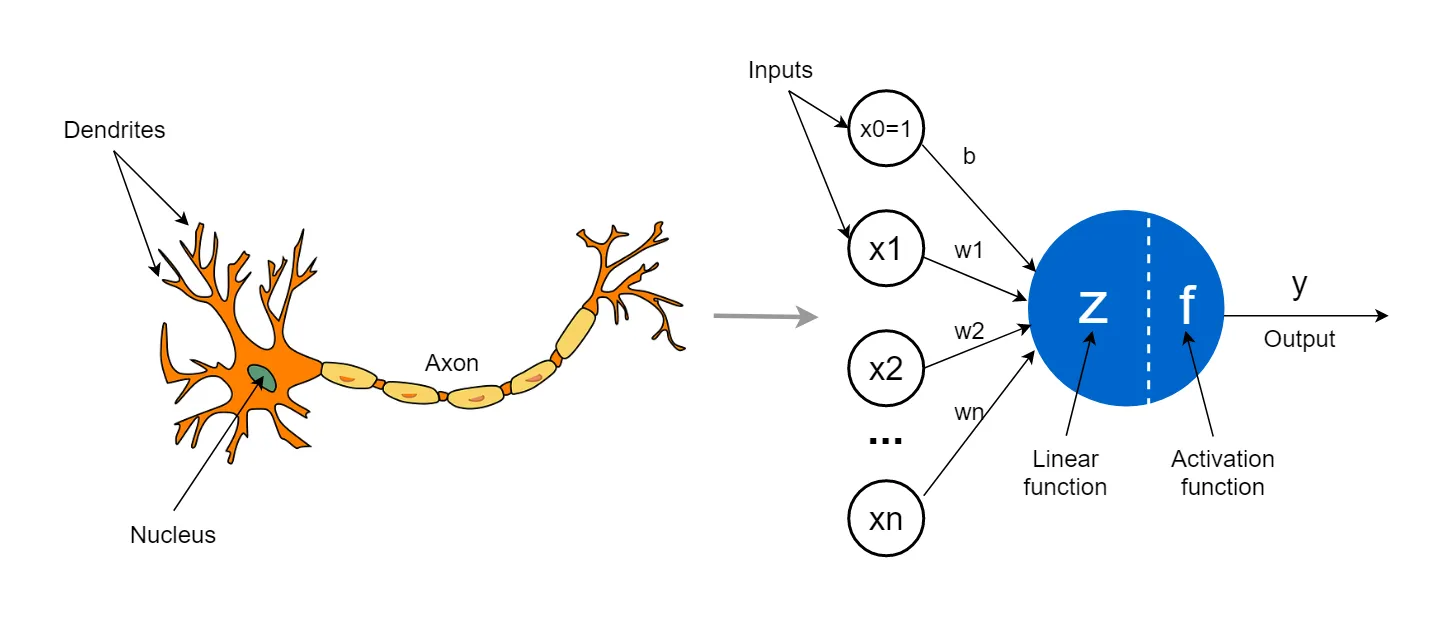
\includegraphics[width=\textwidth]{img/ch1/neuron.png}
    \caption{Illustration of a biological neuron and its analog, the perceptron \cite{pramoditha_concept_2021}.}
    \label{fig:biological-neuron}
\end{figure}

Mathematically, the perceptron abstracts this biological process. The inputs to a perceptron ($x_1, x_2, \ldots, x_n$) are modelled as an input vector $\bm{x}$, where each input represents a dendrite's signal. To represent the strength of the synaptic connection, each input is assigned a weight $w_i$, forming a weight vector $\bm{w}$. The neuron ``fires'' when the weighted sum of the inputs, $\bm{x} \cdot \bm{w}$, exceeds a certain threshold determined by an activation function, $f$. There are many different formulations of activation functions, the simplest perhaps being the unit step function which fires when the weighted sum is non-negative:

\begin{equation}
    a = f(n) = 
    \begin{cases}
        1 & \text{if } n \geq 0 \\
        0 & \text{if } n < 0
    \end{cases}
\end{equation}

Additionally, a bias term $b_i$ is introduced to adjust the firing threshold, and so the perceptron's output is determined by the following equation:

\begin{equation}
a_i = f(\bm{w} \cdot \bm{x} + b_i)
\end{equation}

Note that the perceptron either fires or does not fire -- in other words, its output is binary. This binary output was initially designed for performing simple binary classification tasks, where the input vector $\bm{x}$ would be classified as either a positive or negative instance. However, a key limitation of this model is that it only works when the input data is \textit{linearly separable}. This limitation was famously highlighted in 1972 by Minsky and Papert in their book \textit{Perceptrons} \cite{minsky_perceptrons_1972}, where they demonstrated that the perceptron could not solve the XOR problem, a fundamental logic problem that requires the model to output true when the two inputs are not equal, and false when they are. The inability of perceptrons to learn non-linear relationships was a significant roadblock for early \acrshort{ai} research and was, in-part, one of the causes for the first ``\acrshort{ai} winter'' (1974–1980).

\subsubsection{The origins of deep learning}

The limitations of the perceptron in solving non-linearly separable problems such as XOR prompted the development of more sophisticated models. Researchers realised that deeper architectures, where perceptrons were layered on top of each other, could address the inability for perceptrons to capture non-linear decision boundaries. This led to the development of the \textit{\acrlong{mlp}} (\acrshort{mlp}), which is essentially a network of perceptrons arranged in layers. An \acrshort{mlp} consists of an input layer, one or more hidden layers, and an output layer. Each node in the hidden layers performs a weighted sum of inputs, followed by an activation function, and then passes the result to the next layer. This deeper architecture -- giving rise to the field \textit{\acrlong{dl}} (\acrshort{dl}) -- allows the network to capture non-linear relationships. However, the biggest challenge that arose was figuring out how to train such networks efficiently.

The breakthrough for training \acrshort{mlp}s came with the \textit{backpropagation algorithm}, formalised by Rumelhart, Hinton, and Williams in 1986 \cite{rumelhart_learning_1986}. This algorithm solved the problem of efficiently calculating the gradients required to adjust the weights in a multi-layer network. Backpropagation uses the chain rule of calculus to compute the gradients of the loss function with respect to each weight, allowing the network to perform gradient descent to minimise the error. This technique allowed neural networks to be trained to solve more complex, non-linear problems and was a foundational development for modern \acrlong{dl}.

Another significant advancement in \acrlong{ai} came in the late 1980s and early 1990s with the development of the \acrfull{cnn}, a breakthrough often accredited to LeCun and Bengio \cite{lecun_backpropagation_1989, lecun_convolutional_1995}. \acrshort{cnn}s use convolutional layers which apply filters (or kernels) across an input to extract local features, followed by pooling layers to reduce the dimensionality of the data. This hierarchical structure allows \acrshort{cnn}s to capture complex patterns in data with spatial structure such as images by focusing on local regions \cite[Ch. 9]{goodfellow_deep_2016}. \acrshort{cnn}s became especially effective in domains requiring pattern recognition such as image classification and object detection. For example, LeCun used \acrshort{cnn}s to solve digit recognition tasks, notably developing the LeNet-5 architecture \cite{lecun_gradient-based_1998}, which became the foundation of many modern applications in computer vision.

\subsubsection{The 21st century: big data, big machines, and deep networks}

The 2000s marked a significant shift in \acrlong{ai} and \acrlong{ml}, largely due to the rise of big data. With the advent of the internet and social media, vast amounts of data became available for training \acrlong{ml} models. Two of the most prominent datasets from this era include ImageNet \cite{deng_imagenet_2009} and MS-COCO \cite{lin_microsoft_2014}, which became benchmarks for computer vision tasks and helped in providing the sheer volume of training data needed for complex architectures.

A key technological enabler of these advancements was the introduction of the \acrfull{gpu} in the late 2000s which revolutionised the speed with which models could be trained. Compared to traditional CPUs, \acrshort{gpu}s offered up to 70x faster training times \cite{raina_large-scale_2009}, allowing researchers to explore more complex models with greater efficiency, dramatically accelerating progress across a range of \acrlong{ai} disciplines.

The 2010s were an incredibly transformative period for \acrlong{dl}, especially in \acrshort{cnn} architectures \cite{lecun_deep_2015}. Several key architectures were proposed over the decade including AlexNet in 2012 \cite{krizhevsky_imagenet_2012} which introduced the use of ReLU (Rectified Linear Units) as an activation function and demonstrated the power of using \acrshort{gpu}s for training; VGGNet in 2014 \cite{simonyan_very_2014} which improved upon AlexNet by proposing a simpler architecture, reducing the number of parameters required to obtain feature maps and thus improving convergence time and model performance; and ResNet in 2015 \cite{he_deep_2015} which tackled the vanishing gradient problem in very deep networks by introducing the \textit{residual block}, allowing the network to skip layers during training by introducing skip connections.

The decade was not over yet; in 2017, Vaswani et al. presented the groundbreaking transformer model in their now-canonical paper \textit{Attention Is All You Need} \cite{vaswani_attention_2017}. The key innovation in this model was the self-attention mechanism, which allowed the model to focus on different parts of the input sequence dynamically, enabling it to capture long-range dependencies more effectively than traditional \acrshort{rnn}s and \acrshort{lstm}s. This made it incredibly popular for natural language processing models such as Google's BERT \cite{devlin_bert_2018} and OpenAI's GPT-3 \cite{brown_language_2020}.

Soon, transformers expanded into other domains, including computer vision. The 2020 paper \textit{An Image Is Worth $16\times16$ Words} \cite{dosovitskiy_image_2020} introduced the vision transformer model which adapted transformer architectures to image processing tasks by splitting images into patches (analogous to words in text). This paper showed that transformers can surpass traditional \acrshort{cnn} architectures, however only on the condition that the models are trained on incredibly large datasets (14-300 million images).

In summary, the field of \acrlong{ai} has undergone a rapid evolution in just a short period of time, from early innovations such as the perceptron and backpropagation to the emergence of \acrlong{dl} architectures like \acrshort{cnn}s and, more recently, transformers. With this historical context established, we now turn our focus to the diverse range of classifiers employed in \acrshort{uatr} to better understand how these techniques are applied in real-world scenarios.

\subsection{A review of classification techniques}

This thesis is rooted in the subfield of \acrlong{ml}, a branch of \acrshort{ai} that is generally divided into three main paradigms: \textit{unsupervised learning}, where the system identifies patterns and relationships given data without labelled outputs; \textit{supervised learning}, where the system is provided both input data and corresponding labels and learns to map inputs to outputs; and \textit{reinforcement learning}, where the system learns by interacting with an environment and receiving feedback in the form of rewards or penalties. Supervised learning can further be divided into regression or classification based on whether the goal is to predict a continuous quantity or discrete class labels. \acrshort{uatr} primarily employs supervised classification, where the goal is to classify a given sonar signal into a certain vessel type.

\begin{figure}[t]
    \centering
    \begin{tikzpicture}[]
        % Styles
        \tikzstyle{input} = [rectangle, draw, text centered, minimum width=1.5cm, minimum height=1cm, inner sep=10pt, rounded corners=5pt, line width=1pt]
        \tikzstyle{process} = [rectangle, draw, text centered, minimum width=2.5cm, minimum height=1cm, inner sep=10pt, rounded corners=5pt, line width=1pt]
        \tikzstyle{line} = [draw, thick, ->, >=latex]

        % Top Flowchart
        \node[input, fill=blue!10] (input1) {Input};
        \node[process, right=1.1cm of input1, fill=blue!10] (featureextraction1) {Feature Extraction};
        \node[process, right=1.1cm of featureextraction1, fill=blue!10] (classification1) {Classification};
        \node[input, right=1.1cm of classification1, fill=blue!10] (output1) {Output};

        % Arrows for Top Flowchart
        \path[line] (input1) edge (featureextraction1);
        \path[line] (featureextraction1) edge (classification1);
        \path[line] (classification1) edge (output1);
        
        % Label for Top Flowchart
        \node[above=0.3cm of input1] (mlLabel) {\textbf{Machine Learning}};

        % Bottom Flowchart
        \node[input, below=1.5cm of input1, fill=blue!10] (input2) {Input};
        \node[process, right=1.5cm of input2, fill=blue!10] (combinedprocess) {Feature Extraction + Classification};
        \node[input, right=1.5cm of combinedprocess, fill=blue!10] (output2) {Output};

        % Arrows for Bottom Flowchart
        \path[line] (input2) edge (combinedprocess);
        \path[line] (combinedprocess) edge (output2);

        % Label for Bottom Flowchart
        \node[above=0.3cm of input2] (dlLabel) {\textbf{Deep Learning}};
    \end{tikzpicture}
    \caption{A simplified comparison between machine learning and deep learning architectures, recreated from \cite{neupane_review_2020}.}
    \label{fig:ml-vs-dl}
\end{figure}

There are many types of classifier algorithms (Figure \ref{fig:ml-classifiers-mindmap}). However, perhaps the most important distinction to make here is the difference between using traditional \acrlong{ml} models and modern \acrlong{dl} models (Figure \ref{fig:ml-vs-dl}). Traditional \acrshort{ml} models, such as \acrshort{svm} or \acrshort{knn}, typically rely on manual feature extraction. These models depend on domain expertise to hand-engineer features from sonar signals, which are then fed into a classification algorithm. However, this feature engineering can be rigid and limited, as it struggles to capture complex variations and nuances in highly dynamic underwater environments, leading to reduced reliability when conditions change unpredictably \cite[2]{kamal_deep_2013}. Deep learning architectures, on the other hand, automatically learn relevant features from the raw data through using neural networks that have many hidden layers and more complex connections between them -- hence the term \acrlong{dl} \cite{neupane_review_2020}. Unlike traditional \acrshort{ml} models, \acrshort{dl} systems can process data in an end-to-end manner, eliminating the need for manual feature extraction. Additionally, \acrshort{dl} models are more robust when working with large datasets, as they can leverage the sheer volume of data to improve accuracy and generalise better to new, unseen data. However, while \acrshort{dl} models outperform traditional \acrshort{ml} models in feature extraction and scalability, they require extensive labelled datasets for training and can suffer from overfitting when data is scarce.

\begin{figure}[p]
    \centering
    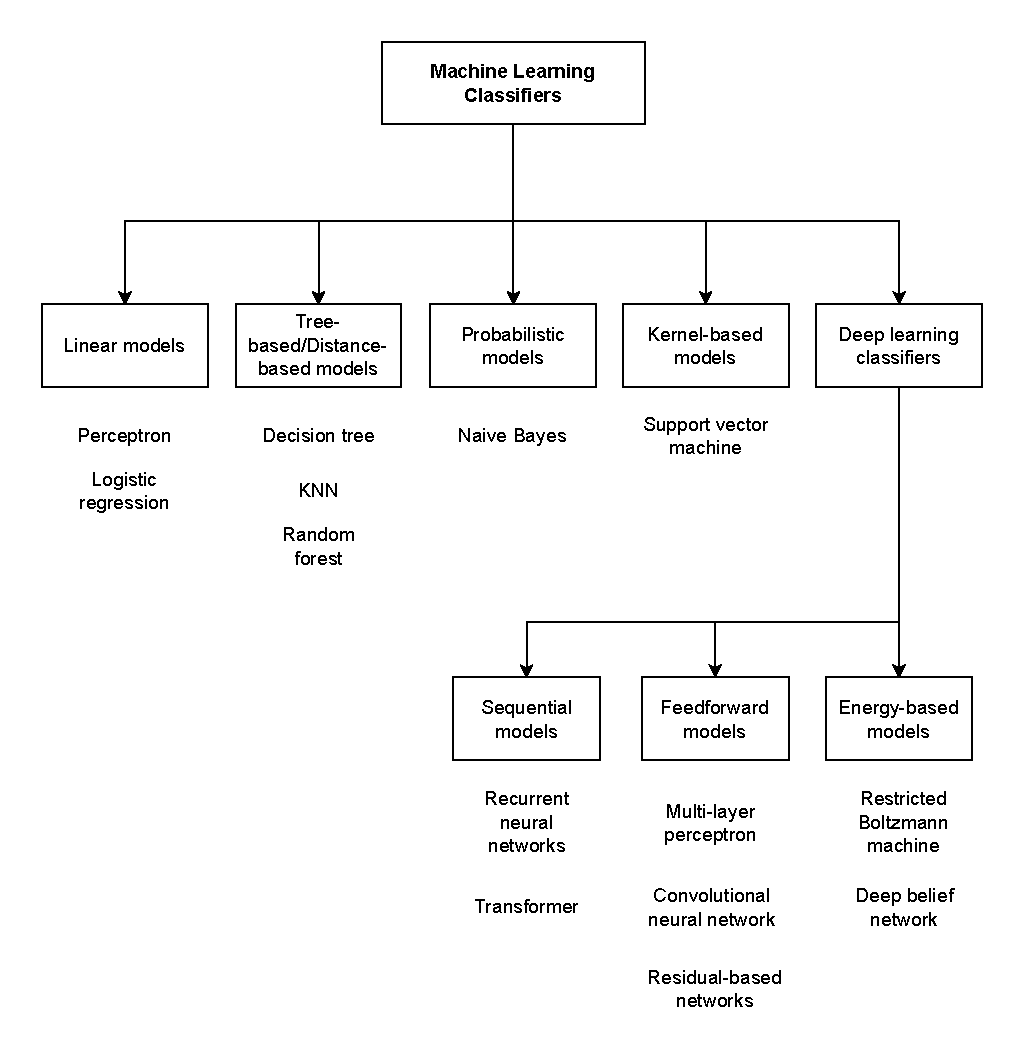
\includegraphics[width=\textwidth]{img/ch2/ml_classifiers.pdf}
    \caption{Categorisation of well-known machine learning classifiers.}
    \label{fig:ml-classifiers-mindmap}
\end{figure}

In this section, we aim to review several key classification techniques used in \acrshort{uatr}, ranging from traditional statistical methods to more modern \acrlong{dl} approaches. In total, over 300 journal articles, conference papers, theses, preprints, and books were collected from various sources including Google Scholar, SemanticScholar, and The University of Sydney library. These were then sorted by citation count to determine the impact of the work. The top 50 pieces of research were then read, reviewed, and summarised for the following literature review \ref{tab:classification-review-summary}.

\begin{sidewaystable}[htbp]
\centering
\begin{tabular}{lllll}
\toprule
\textbf{Paper} & \textbf{Year} & \textbf{Features} & \textbf{Architecture} & \textbf{Dataset} \\ \midrule
Gorman and Sejnowski \cite{gorman_analysis_1988} & 1988 & Spectral envelope & MLP & Proprietary \\
Chin-Hsing et al. \cite{chin-hsing_classification_1998} & 1998 & Wavelet transform & MLP & Proprietary \\
Kamal et al. \cite{kamal_deep_2013} & 2013 & Spectrogram & DBN & Proprietary \\
Wang and Zeng \cite{wang_robust_2014} & 2014 & Hilbert-Huang transform, Bark-wavelet analysis & SVM & Proprietary \\
Sherin and Supriya \cite{sherin_b_m_selection_2015} & 2015 & MFCC & SVM & Proprietary \\
Yue et al. \cite{yue_classification_2017} & 2017 & MFCC & CNN, DBN & Proprietary \\
Cao et al. \cite{cao_convolutional_2019} & 2019 & CQT & CNN & Proprietary \\
Liu et al. \cite{liuUnderwaterTargetRecognition2021} & 2021 & 3-D Mel spectrograms & CRNN & ShipsEar \\
Hong et al. \cite{hong_underwater_2021, hongUnderwaterAcousticTarget2021a} & 2021 & Log-Mel spectrograms, MFCC, CCTZ & Residual-based & ShipsEar \\
Doan et al. \cite{doan_underwater_2022} & 2022 & - & Dense-CNN & Proprietary \\
Feng and Zhu \cite{feng_transformer-based_2022} & 2022 & Mel spectrogram & Transformer & ShipsEar, DeepShip\\ \bottomrule
\end{tabular}
\caption{Summary of high-impact papers in the field of underwater acoustic target recognition.}
\label{tab:classification-review-summary}
\end{sidewaystable}

\subsubsection{Multi-layer perceptron}

The first significant work on using neural networks for sonar signal classification was presented by Gorman and Sejnowski in 1988 \cite{gorman_analysis_1988}. Their neural network model aimed to differentiate between sonar echoes from a metal cylinder and a similarly shaped rock using a dataset of 208 recordings. The network featured 60 input neurons, 2 output neurons, and employed a sigmoid activation function. The experiments explored networks with no hidden layer and those with a single hidden layer (ranging from 2 to 24 units). The spectral envelope was the primary input feature, and after 300 epochs, the network achieved up to 90.4\% accuracy, outperforming a \acrshort{knn} classifier's 82.7\%. The study also highlighted that neural networks could perform comparably to human sonar operators and achieve optimal performance without requiring prior statistical knowledge of the signals.

Building on this, Chin-Hsing et al. \cite{chin-hsing_classification_1998} expanded the feature set for the \acrshort{mlp} model by using the \acrfull{fft} to calculate the average power spectral density and applying wavelet transforms to extract tonal features. The neural network had 256 input units, 64 hidden units, and 2 output classes. The dataset, consisting of signals from three ships at varying speeds, demonstrated a significant accuracy improvement when wavelet-transformed features were used, reaching 96\% compared to 80\% with only power spectral density.

\subsubsection{Support vector machine}

The \acrlong{svm}, introduced by Cortes and Vapnik in 1995 \cite{cortes_support-vector_1995}, is a widely-used classification algorithm that aims to find the \textit{maximum margin hyperplane}, which separates two classes with the largest possible margin. This maximisation ensures the classifier is more robust and generalises well to unseen data. The basic decision rule involves finding the projection of an unknown vector $\bm{u}$ onto a weight vector $\bm{w}$, with the decision boundary given by: 
\begin{equation} 
\sum_i \lambda_i y_i (\bm{x}_i \cdot \bm{u}) + b \geq 0
\end{equation} 
where $\lambda_i$ are Lagrange multipliers, $\bm{x}_i$ are training samples, and $y_i$ are class labels. To handle non-linear data, \acrshort{svm} uses a \textit{kernel trick}, which computes the dot product in a higher-dimensional feature space without explicitly transforming the data, enabling efficient non-linear classification.

As a result, a significant body of research has focused on tuning \acrshort{svm} parameters, such as choosing appropriate kernels and kernel parameters for a given application. For example, in their 2015 paper, Sherin and Supriya \cite{sherin_b_m_selection_2015} focused on optimising \acrshort{svm} parameters for underwater target classification using the BAT algorithm \cite{kacprzyk_new_2010}. The dataset included 114 acoustic signals from four classes -- humpback whale, sea lion, ship, and boat -- processed using \acrshort{mfcc}s for feature extraction. The hybrid kernel approach, which combines linear, polynomial, and radial basis functions, outperformed traditional methods such as particle swarm optimisation, offering a 4\% improvement in classification accuracy. 

%Another seminal paper in the field of \acrshort{uatr} which utilised \acrshort{svm} as its classifier was presented by Wang and Zeng in 2014 \cite{wang_robust_2014}. The paper presents a method for classifying underwater noise signals using a combination of Bark-wavelet analysis (BWA) to improve the \acrlong{snr}, the Hilbert-Huang Transform (HHT) for feature extraction, and \acrshort{svm} for classification. The proposed method was tested on acoustic signals from four different ship classes, and the results demonstrated that the approach significantly outperformed a baseline system without denoising, particularly in noisy environments with lower SNRs. The authors found that the system remained robust under varying noise conditions, achieving higher recognition rates compared to traditional wavelet packet transform methods. This robustness is attributed to the denoising step and the adaptability of BWA and HHT for non-stationary signal processing.

\subsubsection{Deep belief networks}

Kamal et al. explore the use of \acrlong{dbn}s for classifying vessel noise \cite{kamal_deep_2013}. The authors use spectrograms created from a proprietary dataset of 40 vessel recordings as input features for the \acrshort{dbn}. Each \acrshort{rbm} in the \acrshort{dbn} is trained in an unsupervised manner, with progressively abstract features extracted at each layer. Afterward, supervised fine-tuning with backpropagation is performed over 2000 epochs to optimise the model. The \acrshort{dbn} achieved a classification accuracy of 90.23\% demonstrating robust performance in noisy environments. The results highlight the model's ability to capture deep, abstract features and its effectiveness in handling complex ambiances, making deep learning approaches like \acrshort{dbn}s a strong candidate for underwater target recognition.

Yue et al. \cite{yue_classification_2017} evaluate several approaches for classifying underwater acoustic targets, comparing traditional methods like WNDCHRM with classical machine learning models such as \acrshort{mfcc}-\acrshort{svm}, and deep learning models like \acrshort{fft}-\acrshort{cnn} and \acrshort{fft}-\acrshort{dbn}. Using World War II underwater recordings of cruisers, submarines, and torpedoes, the study finds that deep learning models outperform the traditional techniques, with \acrshort{fft}-\acrshort{dbn} achieving the highest accuracy at 96.99\%, followed by 94.75\% for \acrshort{fft}-\acrshort{cnn}, 92.15\% for WNDCHRM and 86.6\% for \acrshort{mfcc}-\acrshort{svm}. The paper emphasises the superior performance of deep learning but notes the challenge posed by the lack of large, labelled datasets in underwater acoustics.

\subsubsection{Convolutional neural networks}

In his 2019 paper \cite{cao_convolutional_2019}, Cao proposed a novel method for classifying underwater targets using \acrshort{cnn}s combined with second-order pooling (SOP) to enhance feature extraction from \acrshort{cqt} representations of radiated acoustic signals. The SOP was designed to capture temporal correlations of different \acrshort{cnn} filters, improving classification accuracy by learning co-occurrences of \acrshort{cnn} features across frequency subbands. Results showed that the proposed \acrshort{cnn}-SOP method outperformed traditional \acrshort{cnn} models using max-pooling, with an 8\% improvement in classification accuracy over state-of-the-art methods. Additionally, the paper found that the \acrshort{cqt} features were more effective than \acrshort{stft} features, yielding better performance with \acrshort{cnn} architectures.

Doan et al.'s 2022 paper \cite{doan_underwater_2022} uses a DenseNet-based deep \acrlong{cnn}, named UATC-DenseNet. The dataset consists of underwater acoustic signals captured by passive sonar in a surveillance system, featuring 12 target classes. The UATC-DenseNet model is designed to process 1D time-series acoustic data by stacking convolutional blocks for feature extraction and employing dense skip connections to facilitate gradient flow and avoid vanishing gradients. The model also incorporates advanced pooling and activation techniques, including exponential linear units (eLU). Through several experiments, the authors demonstrate that larger kernel sizes and deeper networks improve classification accuracy, achieving a classification rate of 99.25\% at 0 dB SNR. 

\subsubsection{Recurrent neural networks}

The 2021 paper by Liu et al. \cite{liuUnderwaterTargetRecognition2021} proposes the use of a convolutional recurrent neural network (CRNN) for \acrshort{uatr}. The authors focus on using a 3-D Mel-spectrogram as the main feature for classification, as it captures both the spectral and dynamic properties of the signal. Data augmentation techniques, including SpecAugment \cite{park_specaugment_2019}, time stretching, pitch shifting, and noise addition, were applied to enhance the dataset and improve the model's generalisation. The CRNN architecture combines \acrshort{cnn}s for local feature extraction and \acrshort{lstm} layers for capturing temporal dependencies in the signal. Tested on the ShipsEar dataset, the CRNN-9 model achieved superior accuracy compared to standalone \acrshort{cnn} and \acrshort{lstm} models, with results showing the CRNN-9 achieving a top classification accuracy of 92.8\%. 

\subsubsection{Residual-based networks}

The journal article \cite{hong_underwater_2021} and conference paper \cite{hongUnderwaterAcousticTarget2021a} presented by Hong et al. propose a residual-based network for \acrshort{uatr}. The authors use the ResNet18 architecture, which is a deep residual network with 18 layers, in tandem with features such as log-Mel spectrogram, \acrshort{mfcc}s, and a combination of chroma, contrast, Tonnetz, and \acrlong{zcr} (CCTZ) to feed into the network. These features are then processed using SpecAugment \cite{park_specaugment_2019} to improve data augmentation. The model was evaluated on the ShipsEar dataset and achieved an impressive classification accuracy of 94.3\%.

\subsubsection{Transformer-based networks}

Feng and Zhu's 2022 paper introduced a new model, the \textit{UATR-Transformer} \cite{feng_transformer-based_2022}, which applied the transformer model to the field of \acrshort{uatr}. The core of the model is built on a transformer architecture inspired by the Tokens-To-Token Vision Transformer. The model processes Mel-spectrogram inputs into T-F tokens which are then processed by a multi-head self-attention layer and further encoded through transformer blocks. For classification, the model replaces the traditional [CLS] token with a novel tokens pooling classifier, which jointly considers relationships between time frames and frequency bins in the spectrogram. The UATR-Transformer achieves superior performance compared to other models with an accuracy of 96.9\% on ShipsEar and 95.3\% on DeepShip. Additionally, the transformer-based architecture demonstrates better computational efficiency, handling the prediction tasks faster than CNN-based models due to its token embedding strategy. 

%DLA solutions have made a lot of recent progress in the modulation classification field. There are still many shortcomings in the existing methods. First of all, the structure of CNN methods is often complex to extract more deep features, which is prone to the overfitting problem resulting in poor practical outcome. The maximum number of Vapnik–Chervonenkis dimensions that the large-scale CNN model can classify training samples is too high. It leads to fitting noise and unrepresentative features in training samples, which makes the model unable to really categorize the true distribution of the whole data. Secondly, it is difficult for the neural network based on RNN, in the main form of long short-term memory (LSTM), to solve the gradient problem after superposition, which is almost impossible to further grow in the recognition effect.
% Underwater acoustic signal classification based on a spatial–temporal fusion neural network (Wang 2024)


\subsection{A review of deep features}\label{subsec:deep-features}

The term ``deep features'' refers to representations that are automatically extracted from input data using deep learning techniques. These features, unlike traditional signal processing methods (Section \ref{sec:traditional-features}), are not hand-crafted by domain experts but are rather learned by the model itself during training. This section delves into the most prominent feature extraction mechanism in modern \acrlong{dl} literature -- encoder-decoder networks -- and specifically focuses on a subset of these networks called \acrlong{ae}s (\acrshort{ae}s).

\subsubsection{Encoder-decoder networks}\label{subsubsection:encoder-decoder}

At its core, an encoder-decoder network is a neural network architecture designed to take some input data, compress it into a simpler form, and then reconstruct the original data from that compressed version. Popularised by Hinton and Salakhutdinov in their seminal 2006 paper \textit{Reducing the Dimensionality of Data with Neural Networks} \cite{hinton_reducing_2006}, these networks are made up of two main parts: the \textit{encoder} and the \textit{decoder}. These parts are typically connected through a middle layer known as the \textit{latent space} or \textit{bottleneck} (Figure \ref{fig:enc-dec-network}).

The encoder's job is to take the input (often an image) and pass it through multiple layers of the network, gradually reducing its size and complexity. The idea is that the encoder learns to pick out the most important features of the input and represent them in a more compact form. This compressed representation is what is stored in the latent space. The decoder then works in reverse. It starts from the compressed information in the latent space and tries to reconstruct the original input data. Essentially, it attempts to ``fill in the blanks'' and generate a complete version of what the input should look like based on the compressed features the encoder identified.

This encoder-decoder structure is extremely useful in feature extraction because it forces the network to learn what aspects of the input are most important. Since the encoder must compress the data, it has to decide which features are essential for accurately reconstructing the input, making it a powerful tool for unsupervised learning tasks like dimensionality reduction, data denoising, or even generating new data.

\begin{figure}[htbp]
\centering
\begin{neuralnetwork}[height=8]
  \tikzstyle{input neuron}=[neuron, fill=orange!70];
  \tikzstyle{output neuron}=[neuron, fill=blue!60!black, text=white];

  \inputlayer[count=8, bias=false, title=Input, text=\xin]

  \hiddenlayer[count=5, bias=false]
  \linklayers

  \hiddenlayer[count=3, bias=false, title={Bottleneck}]
  \linklayers

  \hiddenlayer[count=5, bias=false]
  \linklayers

  \outputlayer[count=8, title=Output, text=\xout]
  \linklayers
\end{neuralnetwork}
\caption{A generic encoder-decoder network.}
\label{fig:enc-dec-network}
\end{figure}

A majority of successful encoder-decoder networks use either fully-connected layers or convolution blocks as their layers. Fully-connected layers (also called dense layers) connect every neuron in one layer to every neuron in the next. These layers are typically used in the latent space and decoder stages of the network to help map learned features from one dimension to another. Fully-connected layers are essential when a model must learn complex, global patterns, but they tend to be less efficient for tasks like image processing, where local features are more relevant. 

It was due to the great computational complexity of dense layers that \textit{convolutional blocks} were conceived, and now form the backbone of many state-of-the-art encoder-decoder networks such as UNet \cite{ronneberger_u-net_2015} and SegNet \cite{badrinarayanan_segnet_2015} (Figure \ref{fig:segnet}). These blocks consist of several key components: 
\begin{enumerate}
    \item Convolution layer: applies the convolution operation to extract features.
    \item Pooling layer: reduces the spatial dimension of the feature maps.
    \item Activation layer: applies a non-linear activation function like ReLU.
    \item Batch normalisation: stabilises and accelerates the training process by normalising activations.
\end{enumerate}

The convolution operation is the core of a convolution block. As mentioned in Section \ref{subsec:ai-history}, the idea of using convolutions for spatial feature extraction was proposed by LeCun in the 1990s \cite{lecun_convolutional_1995} and involves sliding a small filter over the input data to detect patterns, such as edges or textures, by computing dot products between the kernel and overlapping regions of the input. Each filter is capable of detecting a different feature, and as the network deepens, it captures increasingly complex patterns. Convolutional layers reduce the need for fully connected layers because they preserve spatial relationships in the data.

Pooling follows the convolution operation in the block. Pooling is a downsampling technique used to reduce the dimensionality of the feature maps while retaining important information. The most common form is max-pooling, where a window slides over the input feature map and retains only the maximum value from each window, reducing the spatial size of the data. Pooling layers help decrease the computational load and prevent overfitting by summarising the presence of features in a region rather than their exact position.

After pooling, it is common to have an activation function in the convolutional block to introduce non-linearity into the network, enabling the model to learn more complex functions. One of the most commonly used activation functions in convolutional layers is the ReLU (Rectified Linear Unit), which is defined as:
\begin{equation}
    \text{ReLU}(x) = \max(0, x)
\end{equation}

Batch normalisation is the last layer in a convolutional block. Batch norm helps improve the training speed and stability of deep neural networks through normalising the activation output of a layer, ensuring that the data distribution remains consistent throughout the network. This reduces what's known as \textit{internal covariate shift}, where the distribution of activations changes during training making optimisation more difficult. Batch normalisation allows higher learning rates and reduces sensitivity to the initialisation of parameters. Proposed in a 2015 paper \cite{ioffe_batch_2015}, batch norm is applied as:
\begin{equation}
    \hat{x} = \frac{x - \mu}{\sqrt{\sigma^2 + \epsilon}}
\end{equation}
where $x$ is the input, $\mu$ is the mean, $\sigma^2$ is the variance, and $\epsilon$ is a small constant to prevent division by zero. 

The combination of the above operations allows the network to progressively detect more complex patterns in the input data, with each convolutional block learning higher-level features from the previous block's output. 

\begin{figure}[t]
    \centering
    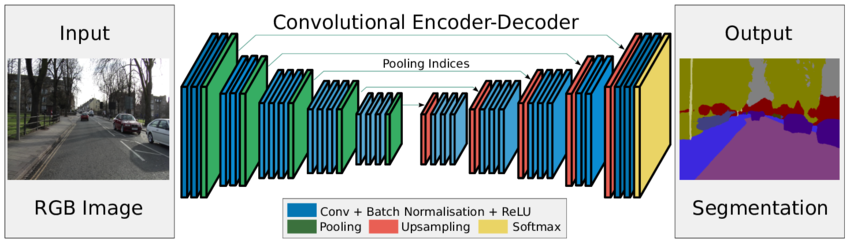
\includegraphics[width=\textwidth]{img/ch1/segnet.png}
    \caption{The SegNet architecture, obtained from \cite{badrinarayanan_segnet_2015}.}
    \label{fig:segnet}
\end{figure}

\subsubsection{Autoencoders}

An \acrlong{ae} is a specialised form of an encoder-decoder network designed primarily for unsupervised learning. Unlike other encoder-decoder networks, \acrlong{ae}s do not have a classifier at the end of the decoder. Instead, they aim to minimise the reconstruction loss when reconstructing the input data from the compressed lower-dimensional latent space. As a result, the encoder is forced to learn which parts of the data are the most important, and the latent space becomes a good lower-dimensional characterisation of the original input \cite{ng_sparse_2010}. \Acrlong{ae}s are widely utilised in tasks such as data dimensionality reduction (acting as a non-linear PCA), denoising, unsupervised feature learning, and even transfer learning, where the learned representations are transferred to other models \cite{goodfellow_deep_2016}.

While there are many variations of autoencoders, there are three key types which are most prominent in the literature: the \acrfull{cae}, the \acrfull{sae}, and the \acrfull{vae}.

\paragraph{Convolutional autoencoder} \acrshort{cae}s are built upon the architecture of \acrshort{cnn}s, but, unlike traditional \acrshort{cnn}s, do not end with a classification layer. Instead, the decoder simply reconstructs the original input. This makes CAEs highly effective for unsupervised learning tasks such as image denoising and anomaly detection. The convolutional layers help in capturing local spatial patterns, making CAEs ideal for handling image or time-series data.

\paragraph{Sparse autoencoder} \acrshort{sae}s introduce a sparsity constraint on the hidden layers of the network, which ensures that only a small number of neurons are active at any given time. This leads the model to learn compact, efficient representations of data, often uncovering more interpretable features. Earlier methods to impose sparsity, such as KL-divergence, aimed to control the average neuron activation relative to a predefined sparsity level. However, more recent approaches like Dropout, introduced by Hinton and Srivastava \cite{hinton_improving_2012, srivastava_dropout_2014}, enforce sparsity more intuitively by randomly deactivating neurons during training, improving generalisation and preventing co-adaptation.

\paragraph{Variational autoencoder} While \acrshort{vae}s share the same encoder-decoder structure, they are designed for generative tasks, where the goal is to generate new data samples rather than merely reconstruct input data. VAEs introduce a probabilistic element to the latent space, learning a distribution over latent variables. Since this paper does not focus on generative models or data generation techniques, the discussion of VAEs will be limited, though they remain a significant area of research in unsupervised representation learning.

A brief review of the most impactful autoencoder-related literature has been provided in Table \ref{tab:ae-review}.

\begin{sidewaystable}
\centering
\begin{tabular}{lllp{4cm}p{11cm}}
\toprule
\textbf{Paper} & \textbf{Year} & \textbf{Architecture} & \textbf{Feature} & \textbf{Notes} \\ \midrule
Bengio et al. \cite{bengio_representation_2013} & 2013 & - & - & Review of key deep feature learning techniques. \\
Xu et al. \cite{xu_stacked_2016} & 2016 & SAE & Image patches & Pioneering work using stacked SAEs for nuclei detection in breast cancer histopathology images. \\
Cao et al. \cite{cao_deep_2016} & 2016 & SAE & Spectrogram & Applied SAE with KL-divergence to enforce sparsity for feature extraction, followed by stacked SAE for classification. \\
Cao et al. \cite{cao_convolutional_2019} & 2018 & SAE & Shaft frequency, WPCE & Built on previous work, integrating features from multiple domains to improve accuracy by 5\%. \\
Chen and Shang \cite{chenUnderwaterTargetRecognition2019} & 2019 & CAE & Spectrogram & Trained CAE on unlabelled noisy samples, followed by fine-tuning with labelled data for classification. \\
Irfan et al. \cite{irfan_novel_2021} & 2020 & CAE & Underwater images & CAE embedded with a softmax classifier for underwater image classification using Fish4Knowledge and ImageNet datasets. \\
Irfan et al. \cite{irfan_deepship_2021} & 2021 & CAE & Mel spectrogram & Introduced the DeepShip dataset and benchmarked it using a CAE model. \\ \bottomrule
\end{tabular}
\caption{A brief literature review of papers using autoencoders for UATR.}
\label{tab:ae-review}
\end{sidewaystable}

%%%%%%%%%%%%%%%%%%%%%%%%%%%%%%%%%%%%%%%%%%%%%%%%%%%%%%%%
\subsection{A review of datasets}

\acrshort{ai} techniques attempt to mimic the human capacity for inductive learning; that is, \acrlong{ml} relies on learning from example \cite{russell_inductive_1991}. The more data you feed into \acrshort{ml} architectures, the better the chance that the program will pick up on the inherent underlying patterns and trends used to correctly classify new examples. Conversely, the program will have a limited accuracy if there are limited examples to learn from \cite{neupane_review_2020}. This property is particularly pronounced in \acrlong{dl} architectures which require an even greater number of training data points in order to reach the desired accuracy and generalisation performance \cite{schmitt_there_2023}. 

Unfortunately, one of the central challenges for \acrshort{ai} researchers in \acrshort{uatr} is the limited availability of suitable data, and this is for multiple reasons:

\begin{enumerate}
    \item Collecting real-world underwater data is resource-intensive and costly, requiring significant time, equipment, logistical coordination, and even legal clearance \cite{irfan_deepship_2021}. It often involves complex setups and the organisation of maritime missions \cite{domingos_survey_2022}.
    \item The curation and annotation of underwater acoustic data is much more specialised compared to other types of data, such as images. While anyone can label images, only trained sonar operators have the expertise to correctly label underwater acoustic signals.
    \item Many underwater acoustic recordings are classified due to defence-related concerns, especially regarding military vessels. This restricts the availability of certain datasets for public use \cite{irfan_deepship_2021, domingos_survey_2022}. For example, the military recordings collected by Zak from five Polish warships in 2008 remain unavailable due to their sensitive nature \cite{zak_ships_2008}.
    \item Underwater recordings are subject to a variety of environmental factors that can affect data quality, such as the engine regime of vessels, local recording conditions, and the acoustic propagation characteristics of the ocean \cite{david_santos-dominguez_shipsear_2016}. Further factors include time of day, season, geographic location, sensor type, depth, and environmental conditions like pressure \cite{domingos_survey_2022, hovem_marine_2012}. Additionally, issues such as weak target signals, non-uniform intensities, and reverberation can further complicate data collection and processing \cite{luo_survey_2023}. High-quality recordings are challenging to capture due to propagation losses -- such as expansion, absorption, and boundary losses -- which make the process time-consuming and energy-intensive \cite{luo_survey_2023}.
\end{enumerate}

Despite these obstacles, researchers have managed to develop several key datasets to support work in underwater acoustic target recognition. Below we have traced out the evolution of these datasets, beginning with foundational private datasets before moving on to ShipsEar \cite{david_santos-dominguez_shipsear_2016}, DeepShip \cite{irfan_deepship_2021}, and two recent contributions in 2024, QiandaoEar22 \cite{du_qiandaoear22_2024} and Oceanship \cite{huang_oceanship_2024}.

\subsubsection{Foundational private datasets}

Most datasets used in underwater acoustics research have traditionally been private, often collected by the researchers themselves. Historically, much of the research in this domain has focused on the characterisation of noise generated by vessels to better understand the impact of various components on sonar signals. One of the foundational studies in this area was conducted by Arveson and Vendittis in 2000, who recorded and analysed the noise radiated from a US coal carrier, identifying the noise contributions of the diesel generator and propulsion-related sources \cite{arveson_radiated_2000}. Similarly, Pricop et al. deployed three hydrophones in the Black Sea to capture ship noise and examined the influence of engines and generators on the vessel's acoustic output \cite{pricop_underwater_2010}. Roth et al. recorded hours of noise data produced by an icebreaker operating in the Arctic, distinguishing between periods of transit and various ice-breaking activities \cite{roth_underwater_2013}. Among the largest privately collected datasets in this field is the work of McKenna et al. who in 2012 recorded and analysed the acoustic emissions from 29 freighters traversing the Santa Barbara Channel, producing a dataset with a total duration of 422 minutes \cite{mckenna_underwater_2012}. 

However, none of the data recorded in these studies is available publicly. Excluding the work by McKenna et al., all datasets were quite small and would only work well for traditional digital signal processing approaches. Furthermore, most of these studies were conducted for purposes other than \acrshort{uatr}, such as noise pollution monitoring. Therefore, the data might not be structured in a way that is useful for vessel classification.

\subsubsection{ShipsEar}

ShipsEar \cite{david_santos-dominguez_shipsear_2016} was published by Santos-Dom\'inguez et al. in 2016 and contains 78 recordings of 39 ships in 11 vessel classes, spanning a duration of 162 minutes and 18 seconds. The authors also included 12 recordings of various ambient noise sources with the view that it would be useful to help discriminate between true signals and background noise, bringing the total dataset length to 181 minutes and 18 seconds. Each recording lasts between 15 seconds to 10 minutes. A detailed breakdown of the database can be found in Table \ref{tab:shipsear-summary}. 

\begin{table}[htbp]
\centering
\begin{tabular}{llll}
\toprule
\textbf{Vessel class} & \textbf{Ships} & \textbf{Recordings} & \textbf{Total recording time (min:s)} \\ \midrule
Dredger       & 1  & 5   & 4:22  \\
Passengership & 7  & 30  & 71:08 \\
Tug boat      & 2  & 2   & 3:26  \\
Ocean liner   & 4  & 7   & 17:02 \\
Motor boat    & 9  & 13  & 18:34 \\
Ro-ro         & 3  & 5   & 15:13 \\
Trawler       & 1  & 1   & 2:43  \\
Pilot ship    & 1  & 2   & 2:18  \\
Sail boat     & 2  & 4   & 6:48  \\
Mussel boat   & 5  & 5   & 12:10 \\
Fish boat     & 4  & 4   & 8:34  \\
Ambient noise & –  & 12  & 19:00 \\ 
\textbf{Total}& \textbf{39} & \textbf{90} & \textbf{181:18} \\ \bottomrule
\end{tabular}
\caption{Summary of the ShipsEar dataset}
\label{tab:shipsear-summary}
\end{table}

Recordings were made off the Spanish Atlantic coast in northwest Spain in autumn 2012 and summer 2013. This location was chosen for its ``intensity and variety of traffic'' given that it is one of the largest fishing ports in the world and also experiences heavy passenger and goods traffic. This allowed the authors to record sonar signals from a variety of vessel classes such as motor boats, sail boats, fishing boats, dredgers etc. The authors also note that because the recordings are from the real environment (as compared to synthetic datasets), the dataset inevitably contains man-made and natural background noise such as from ``waves crashing against the port infrastructure'' and ``occasional vocalisations by marine mammals''.

Each recording was made with a DigitalHyd SR-1 recorder with a sampling rate of 52,734 Hz and a sampling resolution of 24 bits. The bottom of the hydrophone was connected to an underwater buoy to ensure verticality, while the top of the hydrophone was attached to a surface buoy for easy recovery. For depths over 10m, three hydrophones were placed at different depths and with different gains to maximise the dynamic range of the recording (Figure \ref{fig:shipsear-recording}). 

\begin{figure}[htbp]
    \centering
    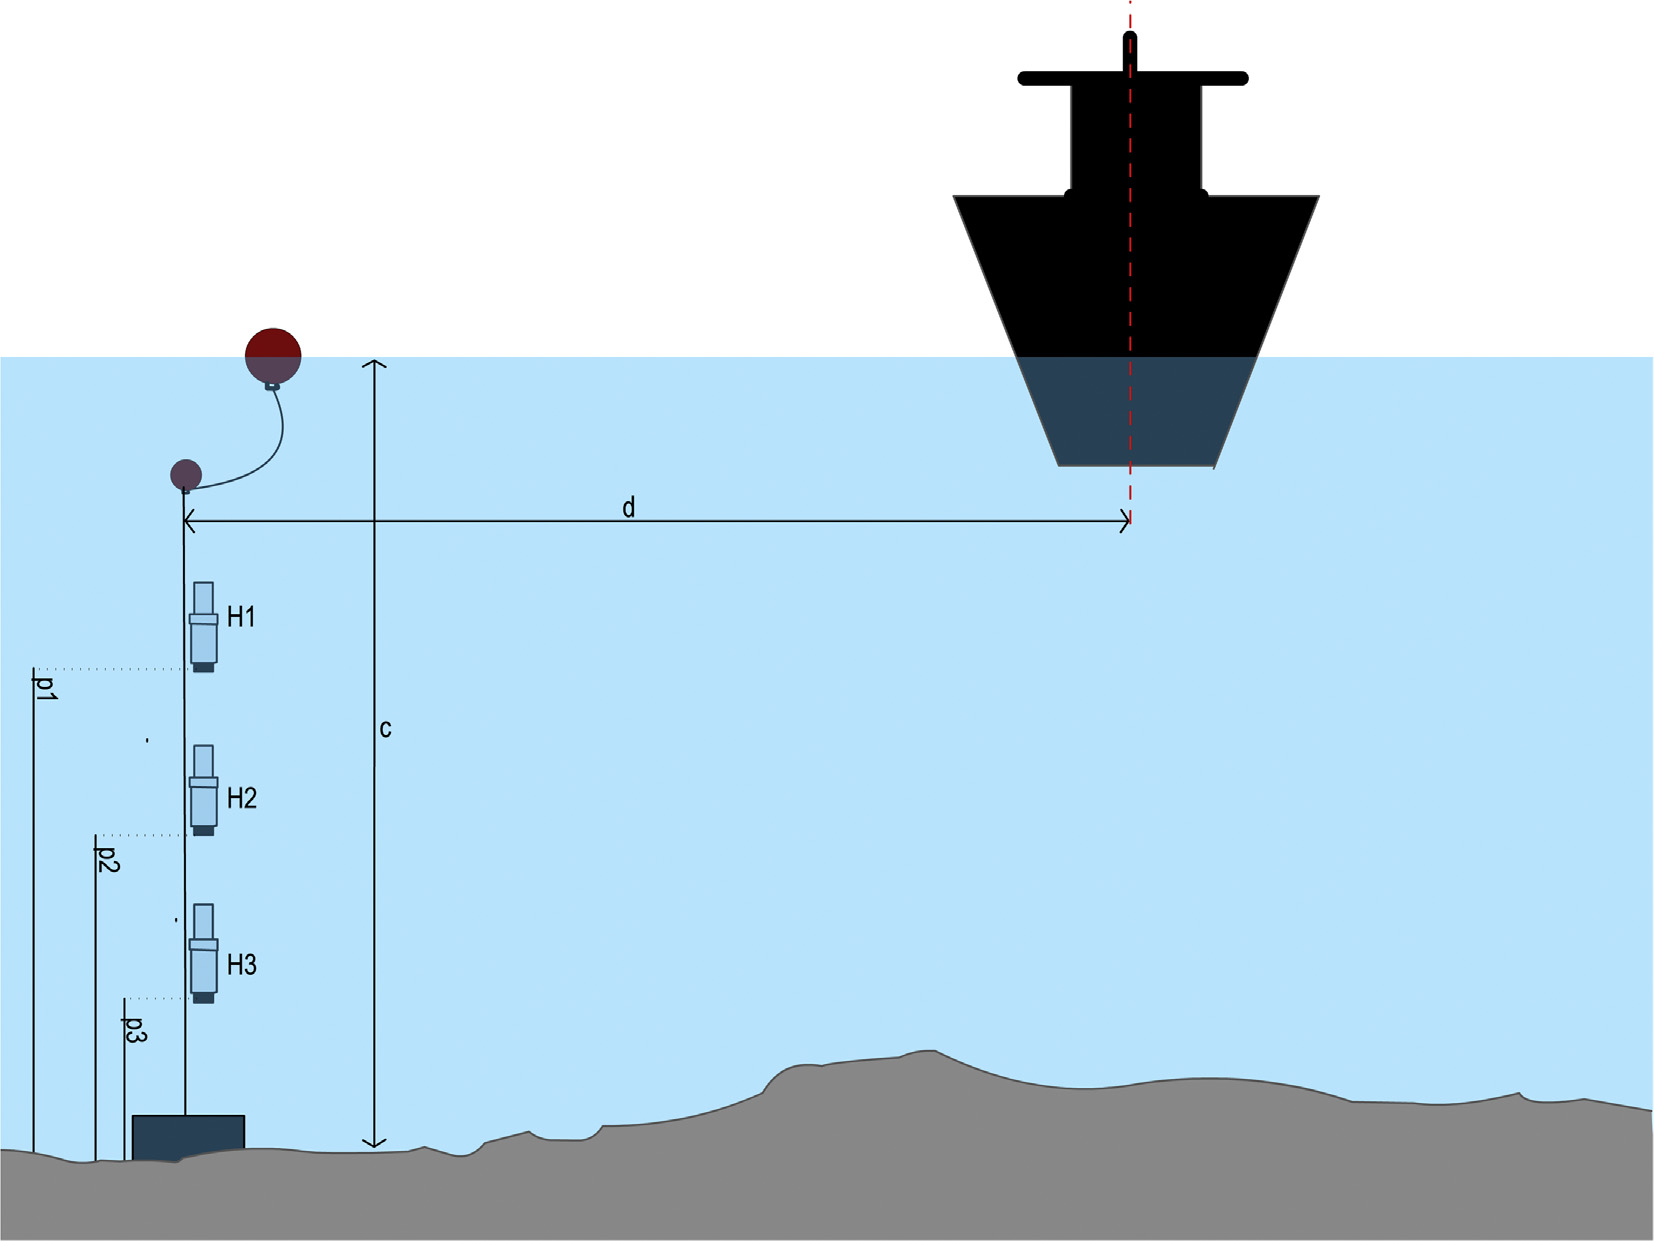
\includegraphics[width=0.6\textwidth]{img/ch2/shipsear_collection.jpg}
    \caption{The recording setup used to create the ShipsEar dataset, obtained from \cite[Fig.~1]{david_santos-dominguez_shipsear_2016}}
    \label{fig:shipsear-recording}
\end{figure}

The database can be viewed at \url{https://underwaternoise.atlanttic.uvigo.es}, where each recording comes with a large amount of metadata including the gains and depths of hydrophones used to record the signal, the approximate distance between the hydrophone and the target vessel, as well as any relevant meteorological data.

Despite its limitations, such as its relatively small volume and class imbalance, the ShipsEar dataset remains a significant contribution to the field of \acrshort{uatr}. With around 3 hours of sonar recordings, it provided a foundation for \acrlong{ml} and signal processing approaches, though not ideal for \acrlong{dl} models which typically require larger datasets to avoid overfitting. The class imbalance issue --- where the largest class (Passengerships) has approximately 31 times more data than the smallest class (Trawler) -- increases this challenge. This is why Santos-Domínguez et al. suggested grouping the original 11 vessel classes into 5 experimental categories; these have since become the standard for research using the dataset (Table \ref{tab:shipsear-merged}).

\begin{table}[htbp]
\centering
\begin{tabular}{lll}
\toprule
\textbf{Class} & \textbf{Vessel classes} & \textbf{Recordings} \\ \midrule
A & Fishing boats, trawlers, mussel boats, tugboats, and dredgers & 17 \\
B & Motor boats, sailboats, pilot boats & 19 \\
C & Passenger ferry & 30 \\
D & Ocean liners and ro-ro ships & 12 \\
E & Background noise & 12 \\ \bottomrule
\end{tabular}
\caption{Experimental classes created for practical use of the ShipsEar dataset}
\label{tab:shipsear-merged}
\end{table}

For over half a decade, ShipsEar remained the largest publicly-available labelled underwater acoustic dataset, enabling great progress in \acrshort{uatr} research and serving as a benchmark for classification tasks in the underwater environment. However, as newer, more extensive datasets have become available, the role of the ShipsEar dataset has become more supplementary than primary in the development of modern \acrshort{uatr} systems.

\subsubsection{DeepShip}\label{subsubsec:deepship}

DeepShip \cite{irfan_deepship_2021}, published by Irfan et al. in 2021, consists of 613 recordings of 265 ships, categorised into four vessel classes, with a total duration of 47 hours and 4 minutes. Each recording ranges from 6 seconds to 25 minutes in length. A detailed breakdown of the database is shown in Table \ref{tab:deepship-summary}.

The recordings were collected over more than two years, from May 2016 to October 2018, in the Strait of Georgia, a busy shipping route located between Vancouver Island and British Columbia, Canada. This area was selected because of its high vessel traffic, allowing the researchers to capture a diverse set of ships across multiple classes.

\begin{table}[htbp]
\centering
\begin{tabular}{llll}
\toprule
\textbf{Vessel class} & \textbf{Ships} & \textbf{Recordings} & \textbf{Total recording time (min)} \\ \midrule
Cargo           & 69  & 110   & 640 \\
Passengership   & 46  & 193   & 742 \\
Tanker          & 133 & 240   & 765 \\
Tug             & 17  & 70    & 677 \\
\textbf{Total}  & \textbf{265} & \textbf{613} & \textbf{2824} \\ \bottomrule
\end{tabular}
\caption{Summary of the DeepShip dataset}
\label{tab:deepship-summary}
\end{table}

Each recording was captured using an icListen AF hydrophone at a sampling rate of 32 kHz, with the depth of the hydrophone ranging between 141 and 147 meters below sea level. Unlike the ShipsEar dataset, which utilised up to three hydrophones, DeepShip used a single hydrophone. To ensure high-quality data, Irfan et al. only recorded when a single vessel was within a 2 km radius of the hydrophone. The dataset is publicly available for download at \url{https://github.com/irfankamboh/DeepShip}.

At present, DeepShip is considered the most comprehensive and authoritative benchmark dataset for \acrshort{uatr} research. It contains nearly seven times the number of recordings as ShipsEar and over 15 times the recording duration, making it an extremely valuable resource for training \acrlong{dl} models in \acrshort{uatr}. Its large volume of data was pivotal in allowing \acrlong{dl} approaches to gain traction in this field, and it provided a common baseline for researchers to compare their results.

One advantage of DeepShip over ShipsEar is that it does not suffer from the same class imbalance problem. The recording times for each vessel class are relatively uniform, which makes it more suitable for classification tasks.

However, a limitation of DeepShip is the restricted nature of its vessel classes and the lack of detailed metadata for individual ships. The four vessel classes -- Cargo, Tug, Passengership, and Tanker -- are broad, and the differences between certain categories, like Cargo and Tanker, may be subtle, as the passive sonar signals generated by their mechanisms are not significantly distinct. This can make classification between these classes challenging and may limit the dataset's generalisability.

\subsubsection{QiandaoEar22}\label{subsubsec:qiandaoear22}

With the issue of data availability in mind, two new underwater acoustic datasets have been published in 2024: QiandaoEar22 and Oceanship. These are both very recently published and have no citations at the time of writing.

QiandaoEar22 \cite{du_qiandaoear22_2024}, published by Du and Hong in May 2024, is a multi-target acoustic dataset consisting of 9 hours and 28 minutes of signal data and 21 hours and 58 minutes of background noise data.

The recordings were taken over four days between the 24th and 28th of June, 2022. The recording locations were off the coast of Houdao (Good Luck) Island in Qiandao (Thousand Island) Lake in China's Zhejiang Province. According to the authors, the recording period coincided with the local tourism season, causing a variety of vessel classes to be recorded such as speedboats, large tour boats, cargo ships, sanitation vessels, small boats, and research ships \cite[5]{du_qiandaoear22_2024}.

The authors used a single DigitalHyd SR-1 hydrophone (the same model used by the ShipsEar team) anchored using a counterweight and buoy system to set its depth. The sampling rate was 52,734 Hz with a sampling resolution of 16 bits. The water depth ranged from 30 to 50 metres and the hydrophone was placed at a depth between 10 and 15 metres. 

Due to QiandaoEar22 being a multi-target dataset, the structure of the dataset is more complex. Each file is in the format:

{\small\centerline{\texttt{YYYYMMDDHHMMSS\_targetType\_name\_distance\_audibility[\&name\_distance\_audibility]*.wav}}}

where:
\begin{itemize}
    \item \texttt{YYYYMMDDHHMMSS} is a 14-digit timestamp (year, month, day, hour, minute, second).
    \item \texttt{targetType} is either \texttt{S} (single target) or \texttt{M} (multiple targets).
    \item \texttt{name} is the concatenated name of the target (alphanumeric characters).
    \item \texttt{distance} is \texttt{F} (far), \texttt{M} (medium), or \texttt{N} (near).
    \item \texttt{audibility} is \texttt{S} (strong), \texttt{M} (middle), or \texttt{W} (weak).
    \item \texttt{[\&name\_distance\_audibility]*} represents optional additional targets, separated by \texttt{\&}, following the same format.
    \item \texttt{.wav} is the file extension.
\end{itemize}

The dataset can be downloaded at \url{https://github.com/xiaoyangdu22/QiandaoEar22}.

QiandaoEar22 offers a much-needed new dataset to the field of underwater acoustics. At a duration of almost nine and a half hours, the dataset sits somewhere in-between ShipsEar and DeepShip in terms of volume. However, the complexity of the multi-target format may present certain challenges. Handling and analysing multiple overlapping sources of noise could complicate data processing and model training. Researchers will need to develop sophisticated methods to separate and classify these signals effectively. It will be interesting to see how the academic and practical applications evolve as researchers utilise this dataset, potentially leading to new insights and advancements in underwater acoustics.

\subsubsection{Oceanship}\label{subsubsec:oceanship}

In August 2024, Li et al. introduced a new dataset into the field of underwater acoustics called Oceanship \cite{huang_oceanship_2024}. The dataset comprises a total of 107,540 recordings, covering 15 vessel classes and spanning 121 hours and 10 minutes in duration. The dataset is divided into two subsets: Oceanship CG (coarse-grained), which contains 53,771 recordings, and Oceanship FG (fine-grained), which includes 53,769 recordings. The key distinction between the two lies in the level of annotation; the fine-grained version provides additional detailed metadata on vessel location, heading, and speed.

Oceanship is essentially a curated compilation of audio recordings sourced from Ocean Networks Canada (\url{https://www.oceannetworks.ca}) captured between 2021 and 2022. The authors decoded Automatic Identification System (AIS)-encoded data to ensure accurate vessel labeling. By adhering strictly to AIS data processing protocols, the dataset ensures high-quality annotations, adding significant value to its use in \acrshort{uatr} tasks.

The scale of Oceanship is particularly noteworthy. The total duration of its recordings is more than twice the length of the DeepShip dataset and over 40 times longer than ShipsEar. This sheer volume of data makes Oceanship the largest publicly available \acrshort{uatr} dataset, offering substantial training data for \acrlong{dl} models.

Another key strength of the dataset is its broad coverage of vessel categories. The 15 classes included in Oceanship account for 83\% of vessel names listed in the AIS naming protocol. These categories also overlap significantly with those used in DeepShip and ShipsEar, which raises the possibility of utilising Oceanship as a pre-training resource for models aimed at classifying vessels in these other datasets. Moreover, the detailed metadata available in Oceanship FG, particularly vessel heading and speed information, offers a level of annotation that is absent in DeepShip, providing researchers with richer data for model development and analysis.

Oceanship has the potential to surpass DeepShip as the benchmark dataset for \acrshort{uatr}. However, at the time of writing, the dataset has yet to be fully accessible to the public. Issues with the uploaded files, particularly the FG subset, have prevented users from downloading the complete dataset. Once these issues are resolved, Oceanship could become an indispensible resource for the \acrshort{uatr} community.

\subsubsection{Challenges}

Despite the availability of datasets like ShipsEar and DeepShip, many researchers continue to rely on proprietary and often confidential datasets, greatly reducing the reproducibility of their results. There are numerous examples of this; for instance, Shin et al. collected 66 minutes of data from a single ship navigating through the Korean Peninsula but noted that, ``because we used passive sonar systems developed for defence purposes, details such as the sampling frequency, sensor array design frequency, sensor distances, and frequency components of the radiation signal cannot be disclosed'' \cite[8]{shin_passive_2022}. 

This lack of transparency is a pervasive issue in the field of \acrshort{uatr}. To assess the extent of this problem, we compiled and reviewed a set of recent papers in the field, categorising them based on whether they utilised proprietary datasets. Out of the 80 papers examined, 54 employed private datasets -- an overwhelming majority. This issue is consistently noted across various reviews in the field, with Aslam et al. \cite[16]{aslam_underwater_2024}, Domingos et al. \cite[24]{domingos_survey_2022}, Neupane and Seok \cite[24]{neupane_review_2020}, Luo et al. \cite[12]{luo_survey_2023}, and Niu et al. \cite[19]{niu_advances_2023} all identifying the lack of data availability as a critical, if not the most pressing challenge facing \acrshort{uatr} research. In fact, Domingos et al. goes as far to say that the lack of common datasets ``renders this type of research largely insubstantial, since without a common body of data, comparing and benchmarking solutions is a virtually impossible task'' \cite[24]{domingos_survey_2022}. They further remark that in order to facilitate reproducibility, both the code and datasets used in journal papers should be made public -- ``otherwise, the very purpose of publishing results is defeated'' \cite[24]{domingos_survey_2022}.

Moreover, even when public datasets are used, inconsistency in how data is divided between training and test sets can significantly skew results. Both DeepShip and ShipsEar serve as valuable benchmarks for research, yet these databases do not enforce a standard method of dividing data, leading to discrepancies in performance metrics across studies. For instance, some researchers divide audio records into multiple segments and assign these segments randomly to training and test sets, which can lead to the same underlying recording being represented in both sets. Since ship-radiated noise tends to remain stable over time, this can cause models to overfit, inflating their performance. To prevent such information leakage, it is recommended that entire audio records be used for either training or testing, but not both. Standardising such data division methods would allow for more rigorous validation and enable more meaningful comparisons across studies \cite{niu_advances_2023}.